\documentclass[letterpaper,12pt,oneside]{article}\usepackage[]{graphicx}\usepackage[]{color}
%% maxwidth is the original width if it is less than linewidth
%% otherwise use linewidth (to make sure the graphics do not exceed the margin)
\makeatletter
\def\maxwidth{ %
  \ifdim\Gin@nat@width>\linewidth
    \linewidth
  \else
    \Gin@nat@width
  \fi
}
\makeatother

\definecolor{fgcolor}{rgb}{0.345, 0.345, 0.345}
\newcommand{\hlnum}[1]{\textcolor[rgb]{0.686,0.059,0.569}{#1}}%
\newcommand{\hlstr}[1]{\textcolor[rgb]{0.192,0.494,0.8}{#1}}%
\newcommand{\hlcom}[1]{\textcolor[rgb]{0.678,0.584,0.686}{\textit{#1}}}%
\newcommand{\hlopt}[1]{\textcolor[rgb]{0,0,0}{#1}}%
\newcommand{\hlstd}[1]{\textcolor[rgb]{0.345,0.345,0.345}{#1}}%
\newcommand{\hlkwa}[1]{\textcolor[rgb]{0.161,0.373,0.58}{\textbf{#1}}}%
\newcommand{\hlkwb}[1]{\textcolor[rgb]{0.69,0.353,0.396}{#1}}%
\newcommand{\hlkwc}[1]{\textcolor[rgb]{0.333,0.667,0.333}{#1}}%
\newcommand{\hlkwd}[1]{\textcolor[rgb]{0.737,0.353,0.396}{\textbf{#1}}}%

\usepackage{framed}
\makeatletter
\newenvironment{kframe}{%
 \def\at@end@of@kframe{}%
 \ifinner\ifhmode%
  \def\at@end@of@kframe{\end{minipage}}%
  \begin{minipage}{\columnwidth}%
 \fi\fi%
 \def\FrameCommand##1{\hskip\@totalleftmargin \hskip-\fboxsep
 \colorbox{shadecolor}{##1}\hskip-\fboxsep
     % There is no \\@totalrightmargin, so:
     \hskip-\linewidth \hskip-\@totalleftmargin \hskip\columnwidth}%
 \MakeFramed {\advance\hsize-\width
   \@totalleftmargin\z@ \linewidth\hsize
   \@setminipage}}%
 {\par\unskip\endMakeFramed%
 \at@end@of@kframe}
\makeatother

\definecolor{shadecolor}{rgb}{.97, .97, .97}
\definecolor{messagecolor}{rgb}{0, 0, 0}
\definecolor{warningcolor}{rgb}{1, 0, 1}
\definecolor{errorcolor}{rgb}{1, 0, 0}
\newenvironment{knitrout}{}{} % an empty environment to be redefined in TeX

\usepackage{alltt}
\usepackage[paperwidth=8.5in,paperheight=11in,top=1in,bottom=1in,left=1in,right=1in]{geometry}
\usepackage{setspace}
\usepackage[colorlinks=true,allcolors=Blue]{hyperref}
\usepackage[usenames,dvipsnames]{xcolor}
\usepackage{indentfirst}
\usepackage{titlesec}
\usepackage{multirow}
\usepackage{booktabs}
\usepackage{graphicx}
\usepackage{verbatim}
\usepackage{rotating}
\usepackage{tabularx}
\usepackage{outlines}
\usepackage{lineno}
\usepackage{array}
\usepackage{times}
\usepackage{cleveref}
\usepackage{acronym}
\usepackage[position=t]{subfig}
\usepackage{paralist}
\usepackage[noae]{Sweave}
\usepackage{natbib}
\usepackage{array}
\usepackage{pdflscape}
\usepackage{bm}
\usepackage{fixltx2e}
% \usepackage{showlabels}
\bibpunct{(}{)}{,}{a}{}{,}

% page margins and section title formatting
\linespread{1.5}
\setlength{\footskip}{0.5in}
\titleformat*{\section}{\Large\bf\em}
\titleformat*{\subsection}{\singlespace\large\bf}
\titleformat*{\subsubsection}{\singlespace\normalsize\bf\em}
\titlespacing{\section}{0in}{0in}{0in}
\titlespacing{\subsection}{0in}{0in}{0in}
\titlespacing{\subsubsection}{0in}{0in}{0in}

% cleveref options
\crefname{table}{Table}{Tables}
\crefname{figure}{Fig.}{Figs.}
\renewcommand{\figurename}{Fig.}

% aliased citations
\defcitealias{LehrterIR}{Lehrter et al. in review}

%acronyms
\acrodef{chla}[chl-\textit{a}]{chlorophyll \textit{a}}
\acrodef{cgem}[CGEM]{Coastal General Ecosystem Model}
\acrodef{do}[O$_2$]{dissolved oxygen}
\acrodef{gom}[GOM]{Gulf of Mexico}
\acrodef{lcs}[LCS]{Louisiana continental shelf}
\acrodef{marb}[MARB]{Mississippi-Atchafalaya River Basin}
\acrodef{zerod}[0-D]{zero-dimensional}
\acrodef{par}[PAR]{photosynthetically active radiation}

%for supplemental figures/tables
\newcommand{\beginsupplement}{%
        \setcounter{table}{0}
        \renewcommand{\thetable}{S\arabic{table}}%
        \setcounter{figure}{0}
        \renewcommand{\thefigure}{S\arabic{figure}}%
     }

%knitr options


% R dependencies


% get the version based on commit date


% get online bib file


\IfFileExists{upquote.sty}{\usepackage{upquote}}{}
\begin{document}

\raggedbottom
\linenumbers
\raggedright
\urlstyle{same}
\setlength{\parindent}{0.5in}
\renewcommand\refname{References \vspace{12pt}}

\begin{singlespace}
\title{{\bf {\Large Parameter sensitivity and identifiability for a biogeochemical model of hypoxia in the northern {G}ulf of {M}exico}}}
\author{
  {\bf {\normalsize Marcus W. Beck$^1$, John C. Lehrter$^1$, Lisa L. Lowe$^2$}}
  \\\\{\textit {\normalsize $^1$USEPA National Health and Environmental Effects Research Laboratory}}
  \\{\textit {\normalsize Gulf Ecology Division, 1 Sabine Island Drive, Gulf Breeze, FL 32561}}
	\\{\textit {\normalsize Phone: 850-934-2480, Fax: 850-934-2401}}
	\\{\textit {\normalsize Emails: \href{mailto:beck.marcus@epa.gov}{beck.marcus@epa.gov}, \href{mailto:lehrter.john@epa.gov}{lehrter.john@epa.gov}}}
	\\\\{\textit {\normalsize $^2$Lockheed Martin IS \& GS - Civil, supporting the USEPA}}
	\\{\textit {\normalsize Resarch Triangle Park, NC 27709}}
	\\{\textit {\normalsize Phone: 919-541-3985,}}
	\\{\textit {\normalsize Email: \href{mailto:lowe.lisa@epa.gov}{lowe.lisa@epa.gov}}}
  \vspace{1in} 
  \\ Version Date:   Wed Aug 24 11:58:31 2016 -0500
	}
\date{}
\maketitle
\end{singlespace}
\clearpage

\begin{abstract}
\noindent Bio-geo-chemical models are useful tools in environmental sciences that can guide management and policy-making. Consequently, significant time and resources are spent developing these models in system-specific contexts. The optimization of model parameters to maximize precision, including transferability of these models to different systems, are fundamental concerns in the development and application of these tools. This study describes quantitative limitations of coupled hydrodynamic-ecological modelling by contrasting numeric and ecological certainty with a systematic framework for characterizing parameter sensitivity and identifability.  We evaluate a simple bio-geo-chemical model that is the \ac{zerod} unit of a larger spatio-temporal model of hypoxia on the \acl{lcs} of Gulf of Mexico as an example. Results from analysis of the \ac{zerod} model are used to infer larger trends in dissolved oxygen dynamics over time, having implications for understanding factors that contribute to environmental conditions that are detrimental to aquatic resources.  In particular, we focus on issues of parameter identifiability using local sensitivity analyses to provide quantitative descriptions of numerical constraints on model precision.  We argue that quantitative and ecological certainty in model calibration are often at odds and the practitioner must explicitly choose model components to optimize given tradeoffs between the two. We further conclude that numerically optimal parameter sets for models of hypoxia are often small subsets of the complete parameter set because of redundancies in the unique effects of paramater perturbations on model output.  As a result, we demonstrate that use of a model for inference into ecological mechanisms of observed or predicted changes in hypoxic condition can be potentially misguided in the absence of quantitative descriptions of identifiability.  Although these concerns have been expressed in the literature, they are rarely explicitly addressed or included in model evaluations.  In addition to immediate implications for regional models, we provide a framework for describing the effects of parameter uncertainty and identifiability that can be applied to similar models to better inform environmental management.
\end{abstract}
\acresetall

\section{Introduction}

Hypoxia formation in bottom waters of coastal oceans occurs primarily from excess nutrient inputs from land-based sources \citep{Justic87,Diaz95,Howarth96}.  These events are detrimental to aquatic organisms and have significant negative effects on economic resources derived from coastal ecosystems \citep{Lipton03,Diaz11}.  An understanding of the biological, physical, and chemical processes that contribute to the growth of hypoxic areas is a critical concern for mitigating and preventing these negative impacts.  Numerical ecosystem models have been important tools for describing current knowledge of ecosystem processes that contribute to hypoxia formation and for predicting the effects of proposed management activities or future scenarios \citep{Scavia04,Hagy07,Pauer16}.  Unlike statistical models that have more generic structures, simulation and process-based models include explicit descriptions of relevant processes that are constrained by empirical or observational data relevant to the system of interest \citep[e.g.][]{Omlin01b,Eldridge10}.  These models are often coupled with hydrodynamic grids to provide spatially-explicit representations of patterns in three dimensions \citep{Warner05,Zhao10,Ganju16}. Combined hydrodynamic and bio-geo-chemical models have been developed specifically to describe hypoxic conditions on the \ac{lcs} in the northern \ac{gom} (\citealt{Fennel13,Obenour15,Pauer16}, \citetalias{LehrterIR}).  This area drains a significant portion of the continental United States through the \ac{marb} and is the second largest hypoxic area in the world \citep{Rabalais02}.  Understanding processes that contribute to the frequency and duration of hypoxic events remains a critical research goal for the region, including the application of process-based models to characterize the current knowledge domain.  

The development and application of a model represents a tradeoff between characteristics expected from the output or provided by the structural components. An idealized model is sufficiently generalizable across systems, provides results that are precise given the inputs, and includes components that are realistic descriptions of actual processes \citep{Levins66}. Given that these characteristics cannot be simultaneously achieved, models are developed in partial dependence of reality and theoretical constructs, completely separate from both, or dependent on one or the other \citep{Morrison99,Ganju16}.  These challenges are analagous to the well-known bias-variance tradeoff in statistical models that balances the competing objectives of over- and under-fitting to an observed dataset. Process-based models are more commonly imbalanced between reality and theory, such that most are over-parameterized in an attempt to completely describe reality \citep{Denman03,Nossent12,Petrucci14}.  Such over-parameterization, including use of excessive structural equations, can have serious implications for practical applications.  Quantitative limitations of over-parameterization are analagous to degrees of freedom in standard statistical models as free parameters cannot be numerically estimated when constrained to an observed dataset \citep{Kirchner06}.  More importantly, over-parameterization can limit use across systems outside of the data domain and impose uncertainty in model predictions as realistic values for every variable may not be known or inaccurately applied from existing studies \citep{Durand02,Refsgaard07,Wade08}. The application of process-based models to describe hypoxia dynamics has not been immune to these challenges and more comprehensive approaches are needed to develop models that more carefully balance theory with reality \citep[e.g.,][]{Snowling01}.  

Standard approaches for uncertainty analysis can be used to begin addressing model complexity issues.  In the most general sense, uncertainty is evaluated relative to the effects of input conditions or the observed data used to calibrate a model, changes in parameter values, or variation in the structural components \citep{Beck87}.  Evaluating parameter uncertainty is by far the most common and simplest means of evaluating model behavior.  Although uncertainty analyses should be integrated throughout model development and application, parameters are more often evaluated post-hoc as a form of `damage control' for further calibration.  This approach is sometimes called inverse modelling where results from sensitivity analyses are used to guide calibration or fit of the developed model to observations (\citealt{Soetaert10}, or confronting models with data, \textit{sensu} \citealt{Hilborn97}).  Parameter sensitivity analysis combined with inverse modelling necessarily involves questions of parameter `identifiability', where only a subset of parameters can be numerically constrained to the data as compared to the entire parameter set.  Redundancies in parameter effects lead to unidentifiable models where optimal solutions may be empirically impossible (i.e., standard algorithms will not converge) or parameter values may be non-unique leading to the right answer for the wrong reason \citep{Kirchner06}.  The concept of identifiable parameter subsets is not foreign to hypoxia or eutrophication models  \citep{Omlin01,Estrada10,Mateus15}, although there is a clear need for greater integration of these concepts in model development \citep{Fasham06}.  Moreover, the inclusion of sensitivity and identifiability analyses in model tuning will require the adoption of selection rules that are context-dependent given the subsets that are possible with large parameter sets \citep[e.g.,][]{Wagener01, Wagener01b}.  

This study describes a parameter sensitivity analysis to evaluate identifiability for a bio-geo-chemical model of hypoxia for the northern \ac{gom}.  We evaluate a simple \ac{zerod} unit of a larger spatial-temporal model to explore relationships between multiple parameter sets and hypoxia dynamics on the \ac{lcs}.  Specifically, we provide empirical results to support the assumption that models are generally over-parameterized and only a finite and smaller subset of the larger parameter set can be optimized for a given research question or dataset.  We provide explicit guidance for choosing such subsets of the parameter space given constraints on identifiability as directly related to sensitivity analyses.  The objectives are to \begin{inparaenum}[1\upshape)]
\item identify the parameters that have the greatest influence on \ac{do} using local sensitivity analysis,
\item quantify the identifiability of subsets of the total parameter space based on sensitivity,
\item and provide a set of heuristics for choosing parameters based on sensitivity, identifiability, and parameter categories, including extension to other state variables provided by the model.
\end{inparaenum}
A final analysis evaluates identifiability relative to structural uncertainty to provide an example of extending these methods to more complex uncertainty assessments.  The optimum parameter space is defined as the chosen subset that represents the maximum number of identifiable parameters.  Here, `optimum' is both a qualitative description based on a research question or management goal and a quantitative objective based on numerical optimization criteria for fitting model output to a calibration dataset.  These results can be used to refine existing models or guide application of models to novel contexts, such as downscaling or application to new environments.  We conclude with a discussion of the implications for hypoxia formation in coastal regions, including management strategies for nutrient reduction and use of mechanistic models to inform decision-making.

\section{Methods}

\subsection{Model description}

Hypoxic events, defined  as $<$2 mg L$^{-1}$ of \ac{do} ($<$ 64 mmol m$^-3$), occur seasonally in bottom waters in the northern \ac{gom}.  The \ac{lcs} receives high nutrient loads from the \ac{marb} that drains a significant portion of the continental United States.  Nutrient-stimulated primary production in surface waters increases biological oxygen demand in bottom waters as sinking organic matter is decomposed \citep{Bierman94,Murrell13}.  The hypoxic area averages 15,540 km$^2$ annually (1993-2015) with minimum concentrations observed from late spring to early fall.  Seasonal variation is strongly related to carbon and nutrient export from the \ac{marb} \citep{Lohrenz08,Bianchi10}, whereas hydrologic variation, currents, and wind patterns can affect vertical salinity gradients that contribute to the formation of hypoxia \citep{Wiseman97,Paerl98,Obenour15}. 

This study evaluated a recently developed hydrodynamic and ecological model that describes horizontal and vertical transport and mixing of state variables relevant for hypoxia in the northern \ac{gom}.  The \ac{cgem} includes elements from the Navy Coastal Ocean Model \citep{Martin00} that describes hydrodynamics on the \ac{lcs} and a biogeochemical model with multiple plankton groups, water-column metabolism, and sediment diagenesis \citep{Eldridge10}.  The hydrodynamic component of \ac{cgem} provides a spatially-explicit description of hypoxia using an orthogonal grid with an approximate horizontal resolution of 1.9 km$^2$ and twenty equally-spaced vertical sigma layers on the shelf (depth $\leq$ 100 m, with additional hybrid layers at deeper depths).  The biogeochemical component includes equations for 36 state variables including six phytoplankton groups (with nitrogen and phosophorus quotas for each), two zooplankton groups, nitrate, ammonium, phosphate, dissolved inorganic carbon, oxygen, silica, and multiple variables for dissolved and particulate organic matter from different sources.  Atmospheric and hydrological boundary conditions described in \citet{Hodur97} and \citet{Lehrter13} are also included in \ac{cgem}.

The core unit of \ac{cgem} is FishTank, a \ac{zerod} model that implements the biogeochemical equations in \citet{Eldridge10} and does not include any form of physical transport (i.e., advection, mixing, or surface flux).  Although FishTank was developed for specific application in \ac{cgem}, it can easily be applied to other hydrodynamic grids. Accordingly, the sensitivity and identifiability analysis described below are informative for both the \ac{lcs} gridded model as well as potential applications to different systems.  The FishTank model provides estimates for the 36 state variables described above using a \ac{zerod} parcel that is uniformly mixed as a closed system.  A set of initial conditions is provided as input to the model that was based on observations of relevant variables obtained from research cruises in April, June, and September 2006 \citep[Table 1 in][]{Murrell14}. 

Results from FishTank are based on time-dependent differential equations that describe energy flow between phytoplankton and zooplankton groups as affected by nutrient uptake rates, organic matter inputs and losses, inherent optical properties, sediment diagenesis, and temperature (\citealt{Penta08,Eldridge10}, see appendix in \citetalias{LehrterIR}).  A total of 108 equations are estimated at each time step to return a value for each of the 36 state variables described by the model.  In addition to the initial conditions, 251 parameter values for each of the equations are also supplied at model execution.  These parameters define relationships among fixed effects in the equations and represent ecological properties described by the model that influence hypoxia formation.  Values for each of the parameters were based on estimates from the literature, field or laboratory-based measurements, or expert knowledge in absence of the former.  As such, a sensitivity analysis of parameter values is warranted given that, for example, literature or field-based estimates may not apply under all scenarios or expert knowledge is not completely certain \citep{Refsgaard07}.



The sensitivity of \ac{do} to perturbations of all relevant parameters for the 108 equations was estimated from January 1\textsuperscript{st} to December 31\textsuperscript{st}, 2006 by running FishTank at a timestep of five minutes. Irrelevant parameters were removed for several reasons; parameters were not relevant for the \ac{zerod} model (i.e., hydrodynamic parameters), were considered physical constants, or had no effect given initial conditions.  Additionally, FishTank includes six phytoplankton and two zooplankton groups to describe complexity in community structure and foodweb dynamics.  However, structural equations for each group are identical such that chosen parameter values primarily control differences between the groups, e.g., large-bodied or small-bodied plankton, slow-growing or fast-growing plankton, etc.  Initial analyses indicated that parameter sensitivity of dissolved oxygen was identical within the six phytoplankton and zooplankton groups.  To remove obvious redundancies in the model, the sensitivity analyses were conducted using only one phytoplankton and one zooplankton group.  The final parameter set that was evaluated included 51 parameters that were further grouped into one of six categories based on applicable biogeochemical components of the model: optics ($n = $ 4 parameters), organic matter (12), phytoplankton (22), temperature (2), and zooplankton (11).  A full description of the model parameters is available as an appendix in \citetalias{LehrterIR}.  

\subsection{Local sensitivity analysis}

The analysis focused on sensitivity of \ac{do} in the \ac{zerod} FishTank model to identify parameters that may affect spatial and temporal variation of hypoxia in the larger model.  A local sensitivity analysis was performed for each of the parameters using a simple perturbation approach to evaluate the change in \ac{do} from the original parameter values.  The analyses relied exclusively on concepts used in the FME package developed for the R statistical programming language \citep{Soetaert10,RDCT16}. Each parameter was perturbed by 50\% of its original value and the model was executed to obtain an estimate of the change in \ac{do}.  For each perturbation, a sensitivity value $S$ was estimated for each time step $i$ given a set value for parameter $j$ as:

\begin{equation} \label{sijeqn}
S_{ij} = \frac{\partial y_i}{\partial \Theta_j}\cdot\frac{w_{\Theta_j}}{w_{y_i}}
\end{equation}

\noindent where the estimate depended on the change in the predicted value for response variable $y$ divided by the change in the parameter $\Theta_j$ multiplied by the quotient of scaling factors $w$ for each.  The scaling factors, $w_{\Theta_j}$ for the parameter $\Theta_j$ and $w_{y_i}$ for response variable $y_i$, were set as the default value of the unperturbed parameter and the predicted value of $y_i$ after perturbation \citep{Soetaert10}.  The scaling ensures the estimates are unitless such that the relative magnitudes allow comparisons of model sensitivity to parameters and state variables that differ in scale.  Sensitivity values for all $j$ parameters were summarized across the time series from $i = 1$ to $n$ as $L1$:

\begin{equation} \label{l1}
L1 = \sum|S_{ij}|/n
\end{equation}

All parameters for each of the six equation categories (optics, organic matter, phytoplankton, temperature, and zooplankton) that had non-zero $L1$ were retained for identifiability analysis.  

\subsection{Identifiability and selecting parameter subsets}

Identifiability of parameter subsets was estimated from the minimum eigenvector of the cross-product of a selected sensitivity matrix \citep{Brun01,Omlin01}:

\begin{equation} \label{gameq}
\gamma = \frac{1} {\sqrt{ \min \left(\rm{EV}[\mathit{\hat{S}}^\top \mathit{\hat{S}}]\right)}}
\end{equation}

\noindent where $\gamma$ ranges from one to infinity for perfectly identifiable (orthogonal) or unidentifiable (perfectly collinear) results for parameters in a sensitivity matrix $S$.  The sensitivity functions were supplied as a matrix $\hat{S}$ with rows $i$ and columns $j$ (\cref{sijeqn}) that described deviations of predicted \ac{do} from the default parameter values.  The matrix $\hat{S}$ was first normalized by dividing by the square root of the summed residuals \citep{Omlin01,Soetaert10}. 

The collinearity index $\gamma$ provides a measure of the linear dependence between sensitivity functions described above for subsets of parameters. Estimates of $\gamma$ greater than 10-15 suggest parameter sets are poorly identifiable \citep{Brun01,Omlin01}, meaning optimal values are inestimable given similar effects of the selected parameters on \ac{do}. Greater sensitivity of a state variable to a subset of parameters does not always imply better identifiability if the individual effects are similar.  An intuitive interpretation of $\gamma$ is provided by \citet{Brun01} such that a change in a state variable caused by a change in one parameter can be offset by the fraction $1 - 1/\gamma$ by the remaining parameters.  That is, $\gamma = 10$ suggests the relative change in \ac{do} for a selected parameter can be compensated for by 90\% with changes in the other parameters. 

Initial analyses suggested that considerably limited subsets of parameters were identifiable of the 51 evaluated for the FishTank model.  Given this limitation, parameter selection must consider the competing objectives of increased precision with parameter inclusion and reduced identifability as it relates to optimization.  An additional challenge is the excessively high number of combinations of parameter sets, which complicates selection given sensitivity differences and desired ecological categories of each parameter.  For example, \cref{fig:combnex} provides a simple graphic of the unique number of combinations that are possible for different subsets of `complete' parameter sets of different sizes (i.e., based on $n$ choose $k$ combinations equal to $n!/\left(k!\left(n-k\right)!\right)$).  The number of unique combinations increases with the total parameters in the set and is also maximized for moderate selections (e.g., selecting half the total).  For example, over 10$^{14}$ combinations are possible by selecting 25 parameters from a set of 50.  Accordingly, parameter selection is complicated by differing sensitivity, identifiability, and the difficulty of choosing from many combinations.

A set of heuristics was developed to balance the tradeoff in model complexity and identifiability given the challenges described above \citep[see also][]{Wagener01}.  These rulesets were developed with the assumption that parameters will be selected with preference for those with high sensitivity and identifability based on $\gamma < 15$ as an acceptable threshold for subsets (e.g., 93\% accountability).  Selection heurestics also recognized that parameter categories (i.e., optics, organic matter, phytoplankton, temperature, zooplankton) may have unequal preferences by model users given questions of interest.  In all selection scenarios, parameters were selected by decreasing sensitivity starting with the most sensitive until identifiability did not exceed $\gamma = 15$ where selections were \begin{inparaenum}[1\upshape)]
\item blocked within parameter category,
\item independent of parameter category,
\item or considering all categories equally.
\end{inparaenum} The selection rules produced seven subsets of parameters that could further be used to optimize model calibration for \ac{do}.

\subsection{Observational and structural uncertainty}

The effects of observational and structural uncertainty on the sensitivity analyses were evaluated for \ac{do}.  These analyses used changes in parameter uncertainty and identifiability to infer the effects of observational and structural uncertainty on model output to create a more comprehensive evaluation.  First, observational uncertainty was evaluated by varying the initial conditions supplied to the model.  The initial conditions were based on observational data from research cruises in the northern \ac{gom} \citep{Murrell14} and uncertainty in these data translates directly to uncertainty that can influence results of the sensitivity analysis.  For example, the sensitivity of \ac{do} to variation in the half-saturation constants for phytoplnakton (the concentration supporting half the maximum uptake rate of nutrients) will vary given the initial nutrient concentrations \citep{Eppley69}.  Further, changes in the ratio between nitrogen and phosphorus could affect sensitivity depending on which nutrient is limiting.  Parameter sensitivity and identifiability was re-evaluated for \ac{do} by varying all initial conditions that were non-zero by 50\% and 200\% of the original values that were estimated from the observed data.  Initial conditions were also changed to test the effects of different limiting nutrients by setting nitrogen and phosphorus values above or below concentrations defined by the standard Redfield ratio.  

The effects of model structure on parameter sensitivity and identifiability were evaluated by including or excluding specific components of the model.  The FishTank model includes several processes that are based on expected conditions or available data.  These `switches' are conceptually different from model parameters as they define the use of explicit equations or processes included in the model structure.  As such, a comparison of sensitivity and identifiability given different equations uses parameter uncertainty to begin addressing componenents of structural uncertainty.  Switches in FishTank include different structural equations for the vertical attenuation of light through the water column (inherent or apparent optical properties, \citealt{Penta09,Eldridge10}) and chlorophyll to carbon ratio models (fixed or dynamic given light and nutrients, \citealt{Cloern95}).  Several switches also affect phytoplankton growth including different models for specific growth and effects of temperature, light dependence, nutrient uptake, and internal cell quotas \citepalias[][references therein]{LehrterIR}.  For simplicity, parameter identifiability was evaluated using three scenarios of simple, intermediate, and complex combinations of model switches.  

The above analyses were repeated for additional state variables estimated by FishTank to provide further descriptions of ecological dynamics that are relevant for hypoxia.  In addition to \ac{do}, other state variables included \ac{chla}, \ac{par}, nitrate, ammonium, particulate organic matter, dissolved organic matter, and phosphorus.  Particulate and dissolved organic matter were estimated as the summation of the respective outputs for organic matter from phytoplankon (\textit{OM1\_A}, \textit{OM2\_A}), fecal pellets (\textit{OM1\_fp}, \textit{OM2\_fp}), river sources \textit{OM1\_rp}, \textit{OM2\_rp}), and boundary conditions (\textit{OM1\_bc}, \textit{OM2\_bc}, see \citetalias{LehrterIR}). 

\section{Results}
%' 
%' % for inline
%' <<echo = FALSE, eavl = F, cache = F>>=
%' data(sens_ests)
%' data(sens_ests_cat)
%' 
%' # number of parameters in each category
%' bycat <- table(sens_ests_cat$Category)
%' nms <- names(bycat)
%' bycat <- as.numeric(bycat)
%' names(bycat) <- nms
%' bycat <- toeng(bycat)
%' 
%' # percent of parameters in each category
%' lncats <- table(sens_ests_cat$Category) %>% 
%'   `/` (table(sort(parcats2(as_df = TRUE)$cats))) %>% 
%'   `*` (100) %>% 
%'   form_fun(nsm_val = 0) %>% 
%'   as.list %>% 
%'   lapply(., paste0, '\\%')
%' 
%' # L1 range
%' sensrng <- with(sens_ests_cat, which(error %in% range(error))) %>% 
%'   sens_ests_cat[., ] %>% 
%'   mutate(
%'     error = sapply(error, scinot),
%'     Parameter = par_txt(Parameter)
%'     )
%' 
%' # L1 range within categories
%' sensrngcat <- split(sens_ests_cat, sens_ests_cat$Category) %>% 
%'   lapply(., function(x){
%'     
%'     with(x, which(error %in% range(error))) %>% 
%'       x[., ] %>% 
%'       mutate(
%'         Parameter = par_txt(Parameter), 
%'         error = sapply(error, scinot)
%'       )
%'     
%'     }
%'   )
%' 
%' # average L1, all and by category
%' sensave <- scinot(mean(sens_ests_cat$error))
%' sensave_cat <- split(sens_ests_cat, sens_ests_cat$Category) %>% 
%'   lapply(., function(x) scinot(mean(x$error)))
%'     
%' # phyto errors
%' phytogrps <- filter(sens_ests_cat, Category == 'Phytoplankton') %>% 
%'   separate(Parameter, c('parm', 'grp'), sep = '_') %>% 
%'   group_by(grp) %>%
%'   summarise(grpave = mean(error)) %>% 
%'   arrange(-grpave) %>% 
%'   mutate(grpave = sapply(grpave, scinot))
%' 
%' # zoop errors 
%' zoopgrps <- filter(sens_ests_cat, Category == 'Zooplankton') %>% 
%'   separate(Parameter, c('parm', 'grp'), sep = '_') %>% 
%'   group_by(grp) %>%
%'   summarise(grpave = mean(error)) %>% 
%'   arrange(-grpave) %>% 
%'   mutate(grpave = sapply(grpave, scinot))
%' @
%' 
%' \subsection{Local sensitivity analysis}
%' 
%' Local sensitivity analyses showed that \ac{do} was sensitive to perturbations in nrow(sens_ests_cat) of 178 parameters (round(100 * nrow(sens_ests_cat)/178, 0)\% of total) in FishTank (see \cref{fig:sensalltile} for other state variables). Within each parameter category, \ac{do} was sensitive to bycat$Optics parameters for optics (lncats$Optics of all optic parameters, \cref{tab:optsens}), bycat$`Organic Matter` for organic matter (lncats$`Organic Matter`, \cref{tab:omsens}), bycat$Phytoplankton for phytoplankton (lncats$Phytoplankton, \cref{tab:phytosens}), bycat$Temperature for temperature (lncats$Temperature, \cref{tab:tempsens}), and bycat$Zooplankton for zooplankton (lncats$Zooplankton, \cref{tab:zoopsens}). Although \ac{do} had the greatest sensitivity to parameters in the zooplankton category (as percentage of total), the relative effects varied. Among all parameters, sensitivity values ranged from $L1 = $ sensrng$error[1] for sensrng$Parameter[1] (tolower(sensrng$Category[1])) to sensrng$error[2] for sensrng$Parameter[2] (tolower(sensrng$Category[2])), whereas average sensitivity among all parameters was $L1 = $ sensave.  Within categories, sensitivity ranged from sensrngcat$Optics$error[1] (sensrngcat$Optics$Parameter[1]) to sensrngcat$Optics$error[2] (sensrngcat$Optics$Parameter[2]) for optics, sensrngcat$`Organic Matter`$error[1] (sensrngcat$`Organic Matter`$Parameter[1]) to sensrngcat$`Organic Matter`$error[2] (sensrngcat$`Organic Matter`$Parameter[2]) for organic matter, sensrngcat$Phytoplankton$error[1] (sensrngcat$Phytoplankton$Parameter[1]) to sensrngcat$Phytoplankton$error[2] (sensrngcat$Phytoplankton$Parameter[2]) for phytopankton, sensrngcat$Temperature$error[1] (sensrngcat$Temperature$Parameter[1]) to sensrngcat$Temperature$error[2] (sensrngcat$Temperature$Parameter[2]) for temperature, and sensrngcat$Zooplankton$error[1] (sensrngcat$Zooplankton$Parameter[1]) to sensrngcat$Zooplankton$error[2] (sensrngcat$Zooplankton$Parameter[2]) for zooplankton (\cref{fig:sensplo}, bottom).  Average sensitivity values in each category were $L1 = $ sensave_cat$Optics for optics, sensave_cat$`Organic Matter` for organic matter, sensave_cat$Phytoplankton for phytoplankton, sensave_cat$Temperature for temperature, and sensave_cat$Zooplankton for zooplankton.  Within the six phytoplankton groups, \ac{do} was sensitive to the same parameters within each group although the sensitivity magnitudes varied. Average sensitivity across parameters in each phytoplankton groups showed that \ac{do} was most sensitive to the first and third phytoplankton groups (average $L1 = $ phytogrps[1, 2], phytogrps[2, 2]), whereas sensitivity to parameters in the remaining groups was much lower (all with average $L1 < 1$). Sensitivity of \ac{do} did not vary considerably between parameters in the two zooplankton groups (average $L1 = $ zoopgrps[1, 2], zoopgrps[2, 2] for groups one and two).
%' 
%' Response of \ac{do} to parameter perturbations was not uniform across the time series.  \Cref{fig:sensplo} shows variation for the top parameters within each category.  Because FishTank does not include a spatial component, the estimated \ac{do} trend describes a closed, heterotrophic system where respiration processes eventually remove all \ac{do} from the model space.  The initial decrease in the time series reflects change from the initial conditions outside of the growing seasons (i.e., January, February), the spring/summer increase represents production associated with expected seasonal growth, and the remaining time series from August to the end of year shows complete removal of \ac{do} as respiration processes dominate metabolic activity. Although this time series is not a realistic depiction of an actual system, the biogeochemical model behaves as expected in the absence of the hydrodynamic model.  Accordingly, the interpretation of sensitivity results from the simple model has relevance in an ecological context.  As expected, parameter perturbations had the largest effect during the summer months, although the effects varied.  An inrease in 50\% from the parameter default values generally caused a reduction in \ac{do} during the summer, with the exception of the zooplankton parameter, sensrngcat$Zooplankton$Parameter[2], which caused an increase in \ac{do}.  The phytoplankton parameter, sensrngcat$Phytoplankton$Parameter[2], had the largest effect such that the \ac{do} time series was similar to the default output in April/May, whereas a dramatic decrease was observed in the remaining months.  The effects of perturbations early in the time series (January, February) showed similar patterns such that a reduction in \ac{do} was most common, particularly for the optics (sensrngcat$Optics$Parameter[2]) and phytoplankton (sensrngcat$Phytoplankton$Parameter[2]) parameters.
%' 
%' \subsection{Subset identifiability}
%' 
%' <<eval = F>>=
%' data(cat_ident)
%' data(top_ident)
%' 
%' # percent combos less than gamma 15, 10 by category
%' collcatpers <- lapply(cat_ident, function(x){
%'   
%'   colls <- x$coll
%'   l15 <- scinot(100 * sum(colls < 15)/length(colls), digits = 1)
%'   l10 <- scinot(100 * sum(colls < 10)/length(colls), digits = 1)
%'   c(l15, l10)
%'   
%'   })
%' 
%' # percent combos less than gamma 15, 10 by top in each category
%' colltoppers <- lapply(top_ident, function(x){
%'   
%'   colls <- x$coll
%'   l15 <- scinot(100 * sum(colls < 15)/length(colls), digits = 1)
%'   l10 <- scinot(100 * sum(colls < 10)/length(colls), digits = 1)
%'   c(l15, l10)
%'   
%'   })
%' 
%' maxtempcoll <- scinot(max(cat_ident$Temperature$coll))
%' @
%' 
%' The identifiability analyses suggested that most parameter subsets exceeded the thresholds of $\gamma = 10, 15$, providing further justification for using selection heuristics for parameter optimization.  Parameter identifiability (as $\gamma$) increased at different rates depending on the parameter category or the number of top parameters that were selected (\cref{fig:identbox}).  By category, identifiability was lowest for parameter subsets in the phytoplankton (collcatpers$Phytoplankton[1]\% less than $\gamma = 15$, collcatpers$Phytoplankton[2]\% less than $\gamma = 10$)  and zooplankton categories (collcatpers$Zooplankton[1]\%, less than $\gamma = 15$, collcatpers$Zooplankton[2]\%, less than $\gamma = 10$), whereas a majority of combinations for temperature were identifiable (collcatpers$Temperature[1]\% less than $\gamma = 15$, collcatpers$Temperature[2]\%, less than $\gamma = 10$).  All subset combinations for optics and organic matter parameters had $\gamma < 10$.  All parameter subsets for choosing the top, top two, and top three parameters in each category were identifiable (\cref{fig:identbox}), whereas a majority were identifiable for choosing the top four (colltoppers$top4[1]\% less than $\gamma = 15$, colltoppers$top4[2]\% less than $\gamma = 10$) and top five (colltoppers$top4[1]\% less than $\gamma = 15$, colltoppers$top4[2]\%, less than $\gamma = 10$) parameters.  
%' 
%' <<eval = F>>=
%' temp_coll <- par_txt(c('Tref(nospA+nospZ)_1', 'Tref(nospA+nospZ)_2', 'Tref(nospA+nospZ)_3', 'Tref(nospA+nospZ)_4', 'Tref(nospA+nospZ)_5', 'Tref(nospA+nospZ)_6', 'Tref(nospA+nospZ)_7', 'Tref(nospA+nospZ)_8'))
%' @
%' 
%' A comparison of average and median identifiability by parameter category and top parameters in each category suggested that individual parameters had large effects on $\gamma$ (\cref{fig:identbox}).  For example, a consistent increase in average $\gamma$ from 2 to 7 parameters in a combination for temperature was observed, whereas median identiability remained low until 6 parameter combinations were evaluated.  Further evaluation showed that identifiability was greatly affected by the inclusion of one or two specific parameters in a subset combination.  \Cref{fig:excltemp} shows the temperature collinearity ($\gamma$) ranges in detail for the parameter subsets in \cref{fig:identbox} before and after excluding individual parameters.  Collinearity increases with more parameters included in a subset, although the increase varies depending on the specific parameter.  Exclusion of the parameters temp_coll[2] and temp_coll[5] showed that $\gamma$ remained well below the 10, 15 threshold for all parameter combinations.  Morever, inclusion of temp_coll[1], temp_coll[4], temp_coll[7], and temp_coll[8] generally reduced collinearity relative to when the parameters were excluded.  Similar analyses identified parameters in other categories that had disproportionate effects on identifiability if included in a subset (see supplementary information).
%' 
%' <<eval = F>>=
%' data(p1z1cat_ident)
%' data(p1z1top_ident)
%' 
%' # percent combos less than gamma 15, 10 by category
%' p1z1collcatpers <- lapply(p1z1cat_ident, function(x){
%'   
%'   colls <- x$coll
%'   l15 <- scinot(100 * sum(colls < 15)/length(colls), digits = 1)
%'   l10 <- scinot(100 * sum(colls < 10)/length(colls), digits = 1)
%'   c(l15, l10)
%'   
%'   })
%' 
%' # percent combos less than gamma 15, 10 by top in each category
%' p1z1colltoppers <- lapply(p1z1top_ident, function(x){
%'   
%'   colls <- x$coll
%'   l15 <- scinot(100 * sum(colls < 15)/length(colls), digits = 1)
%'   l10 <- scinot(100 * sum(colls < 10)/length(colls), digits = 1)
%'   c(l15, l10)
%'   
%'   })
%' @
%' 
%' Comparison of identifiability between categories showed that phytoplankton and zooplankton had the least identifiable parameter subsets.  As noted above, FishTank includes six phytoplankton and two zooplankton groups to characterize community structure and foodweb dynamics that likely have an important role in hypoxia development.  However, structural equations for each group do not vary considerably such that variation in parameter values primarily control differences between the groups, e.g., large-bodied vs small-bodied plankton, slow-growing vs. fast-growing plankton.  To obtain identifiability estimates of the plankton categories that were independent of groups, the identifiability analyses were re-evaluated using only one phytoplankton and one zooplankton group (\cref{fig:p1z1identbox}). Compared to all groups, evaluating a single group improved identifiability such that a majority of parameter combinations were below the threshold (p1z1collcatpers$Phytoplankton[1]\% less than $\gamma = 15$, p1z1collcatpers$Phytoplankton[2]\% less than $\gamma = 10$ for Phytoplankton; p1z1collcatpers$Zooplankton[1]\%, less than $\gamma = 15$, p1z1collcatpers$Zooplankton[2]\%, less than $\gamma = 10$ for zooplankton).  Analysis of identifiability for top parameters in all categories did not show similar changes in identifiability.  Although all combinations for the top one, two, and three parameters in each category were still well below the threshold, selecting the top four and five parameters showed an increase (p1z1colltoppers$top4[1]\% less than $\gamma = 15$, p1z1colltoppers$top4[2]\% less than $\gamma = 10$) and a decrease (p1z1colltoppers$top5[1]\% less than $\gamma = 15$, p1z1colltoppers$top5[2]\% less than $\gamma = 10$) in identifiability, respectively (\cref{fig:p1z1identbox}), compared to results that included all phytoplankton and zooplankton groups (\cref{fig:identbox}).  
%' 
%' \subsection{Parameter selection}
%' 
%' <<eval = F>>=
%' data(tocal)
%' 
%' # n parms and ident for each selection heuristic
%' h1_id <- tocal$cat %>% 
%'   split(., .$Category) %>% 
%'   lapply(function(x){
%'     x <- x[x$coll < 15, ]
%'     list(nrow(x), scinot(max(x$coll), digits = 1))
%'   }) 
%' h2_id <- filter(tocal$top, coll < 15) %>%
%'   list(nrow(.), scinot(max(.$coll), digits = 1)) %>% 
%'   .[c(2, 3)]
%' h3_id <- filter(tocal$cattop, coll < 15) %>%
%'   list(nrow(.), scinot(max(.$coll), digits = 1)) %>% 
%'   .[c(2, 3)]
%' 
%' # which parameter broke selection for h2, h3
%' h2_brk <- tocal$top
%' sel <- which(h2_brk$coll < 15)
%' h2_brk <- h2_brk[c(sel, rev(sel)[1] + 1), ] %>% 
%'   arrange(-coll) %>% 
%'   .[1:2, ] %>% 
%'   list(c(as.character(.$Parameter[1]), .$coll)) %>% 
%'   .[[2]]
%' # which parameter broke selection for h2, h3
%' h3_brk <- tocal$cattop
%' sel <- which(h3_brk$coll < 15)
%' h3_brk <- h3_brk[c(sel, rev(sel)[1] + 1), ] %>% 
%'   arrange(-coll) %>% 
%'   .[1:2, ] %>% 
%'   list(c(as.character(.$Parameter[1]), .$coll)) %>% 
%'   .[[2]]
%' @
%' 
%' Each of the three selection heuristics (blocked by parameter category, independent of category, all categories equally) for \ac{do} differed in the number of selected parameters and distribution of parameters within each category (if applicable, \cref{fig:heurist,tab:identall1}).  For the first selection heuristic, all sensitive parameters from the optics ($n = $ scinot(h1_id$Optics[[1]], digits = 0), $\gamma =$  h1_id$Optics[[2]]) and organic matter ($n = $ scinot(h1_id$`Organic Matter`[[1]], digits = 0), $\gamma =$  h1_id$`Organic Matter`[[2]]) categories were selected, whereas toeng(h1_id$Phytoplankton[[1]])[[1]] were selected for phytoplankton ($\gamma = $ h1_id$Phytoplankton[[2]]), toeng(h1_id$Temperature[[1]])[[1]] for temperature ($\gamma = $ h1_id$Temperature[[2]]), and toeng(h1_id$Zooplankton[[1]])[[1]] for zooplankton ($\gamma = $ h1_id$Zooplankton[[2]]).  For the second selection heuristic, toeng(h2_id[[1]])[[1]] parameters were selected ($\gamma = $ h2_id[[2]], with a majority from the phytoplankton category, \cref{tab:identall1}).  For the third heuristic, toeng(h3_id[[1]])[[1]] parameters were selected ($\gamma = $ h3_id[[2]]) with equal representation between categories. For the second and third selection heuristics, an individual parameter caused a disproportianate increase in $\gamma$ that forced the selection to stop.  Selection independent of category showed that including par_txt(h2_brk[1]) caused in increase in $\gamma$ from scinot(h2_brk[3], digits = 1) to scinot(h2_brk[2], digits = 1) and equal selection within cateogies showed that including par_txt(h3_brk[1]) caused in increase in $\gamma$ from scinot(h3_brk[3], digits = 1) to scinot(h3_brk[2], digits = 1).  Finally, parameter selection for other state variables (\ac{chla}, \ac{par}, nitrate, ammonium, particulate organic matter, dissolved organic matter, phosphorus) also showed that a limited number of parameters were identifiable (for brevity, only results using the second set of selection heuristics are shown, \cref{fig:heurist_stts,tab:identall2}).  Less than ten parameters were selected for each of the remaining state variables with most selected from the phytoplankton category.  Interestingly, no parameters from the temperature category were selected.  

\section{Discussion}

% back of envelop calcs for number of relevant parms, all state variables

We showed only small subsets are identifiable, similar conclusions have been described by citations in \citep{Wagener01}, p. 14 for models that follow traditional calibration schemes (e.g., objective function minimization).

Emphasize that parameters that have the greatest effect on collinearity are not those that have the highest sensitivity (contrast the identifiability by category vs identifiability by top parameters)  , also note that groups of parameters together can have large effects on collinearity, maybe some kind of bootstrap analysis could be done looking at doubletons, etc. The example in teh results highlights how redundant variables can be identified as a necessary part of the model calibration process.

Why did identifiability decrease for top five parameters in each category after removing redundant phyto/zoop groups?

\citep{Denman03} describes over-parameterization for multiple phyto groups, use this to emphasize collinearity issues with the phyto groups despite differing sensitivity values between groups

Identifiability by category - varies with number of parameters in the category but some were more redundant than others (phytoplankton).  

Questions specific to GOM - what initial conditions are important? How many phytoplankton groups do we need (e.g., related to structural uncertainty)?

How does the assimilation of additional parameters (e.g., other state variables) during calibration influence the conclusions?  \citet{Wagener01} describes this as a potential approach to improving model performance by improving the availability of information for model calibration (p. 14).  

How does uncertainty translate to what a model should provide (generality v precision)?  The first step - find out what can be optimized but then do not overfit....

What about structural uncertainty - does sensitivity of a model to variation in a parameter imply parameter uncertainty and/or structural uncertainty?

A final point about optimization with identifiable parameter sets - optimization to fit the data still does not ensure a correct model.  Failing in one way can be over-compensated by another feature, e.g., the parameter set that is optimized (see \cite{Flynn05}, p. 1207, third paragraph), also \citep{Durand02,Arhonditsis08}, also note that over-parameterized models are not necessarily bad, see \citep{Omlin01}, models must be validated for the uses which they were intended where a comparison of observed and predicted is the simplest approach and other methods should be used depending on analysis needs \citep{Rykiel96}

\cite{Omlin01} state that the sensitivity, identifiability, estimation process is iterative (p. 113), need to rinse and repeat for proper calibration. 

How to improve identifiability - get more/better observed data, include obs from other state variables in RSS minimization (eqn q in \cite{Omlin01})

Alternative methods for uncertainty analysis - bayesian, MCMC, nonlinear calibration-constrained optimization \citep{Gallagher07}, \citep{Arhonditsis08}

Our heuristic products are partially analogous to the Rainfall-Runoff Modelling Toolbox (RRMT) presented by \citep{Wagener01b}2001 (cited on page 15, in \citealt{Wagener01}), although ours is simple in comparison

\clearpage
\begin{singlespace}
\bibliographystyle{apalike_mine}
\bibliography{refs}
\end{singlespace}
\clearpage

%%%%%%
% tables

% do sensitivity all categories
%latex.default(totab, file = "", rowlabel = "Description", caption = cap.val,     caption.loc = "top", rowname = Description, rgroup = unique(cats),     n.rgroup = as.numeric(table(cats)), size = tabsize, label = paste0("tab:",         tablab))%
\begin{table}[!tbp]
{\footnotesize
\caption{Sensitivity of \ac{do} to perturbations of indivividual parameters.  Sensitivities are based on a 50\% increase from the initial parameter value, where $L1$ summarizes differences in model output from the default (see \cref{l1}).  Parameters that did not affect \ac{do} are not shown.  Parameters are grouped by categories as optics, temperature, phytoplankton, zooplankton, and organic matter.\label{tab:dosens}} 
\begin{center}
\begin{tabular}{llll}
\hline\hline
\multicolumn{1}{l}{Description}&\multicolumn{1}{c}{Parameter}&\multicolumn{1}{c}{Value}&\multicolumn{1}{c}{L1}\tabularnewline
\hline
{\bfseries Optics}&&&\tabularnewline
~~Chla specific absorption at 490 nm&\textit{astar490}&$0.04$&$6.27\times 10^{-4}$\tabularnewline
~~OMA specific absorption at 490 nm&\textit{astarOMA}&$0.1$&$3.22\times 10^{-4}$\tabularnewline
~~OMZ specific absorption at 490 nm&\textit{astarOMZ}&$0.1$&$5.35\times 10^{-6}$\tabularnewline
\hline
{\bfseries Temperature}&&&\tabularnewline
~~Optimum temperature for growth(C)&\textit{Tref(nospA+nospZ)}&$22$&$1.8\times 10^{-4}$\tabularnewline
\hline
{\bfseries Phytoplankton}&&&\tabularnewline
~~phytoplankton carbon/cell&\textit{Qc}&$1.35\times 10^{-6}$&$0.71$\tabularnewline
~~initial slope of the photosynthesis-irradiance relationship&\textit{alpha}&$8.42\times 10^{-17}$&$0.03$\tabularnewline
~~mortality coefficient&\textit{mA}&$0.1$&$0.03$\tabularnewline
~~N-uptake rate measured at umax&\textit{vmaxN}&$4.1\times 10^{-8}$&$0.03$\tabularnewline
~~coefficient for non-limiting nutrient&\textit{aN}&$1$&$0.01$\tabularnewline
~~phytoplankton basal respiration coefficient&\textit{respb}&$0.02$&$0.01$\tabularnewline
~~half-saturation constant for P&\textit{Kp}&$2.86$&$0.01$\tabularnewline
~~minimum N cell-quota&\textit{QminN}&$6.08\times 10^{-9}$&$7.44\times 10^{-3}$\tabularnewline
~~maximum growth rate&\textit{umax}&$0.41$&$5.34\times 10^{-3}$\tabularnewline
~~half-saturation constant for N&\textit{Kn}&$4.51$&$1.56\times 10^{-3}$\tabularnewline
~~P-uptake rate measured at umax&\textit{vmaxP}&$2.68\times 10^{-8}$&$1.3\times 10^{-3}$\tabularnewline
~~minimum P cell-quota&\textit{QminP}&$6.19\times 10^{-10}$&$1.59\times 10^{-4}$\tabularnewline
~~phytoplankton growth respiration coefficient&\textit{respg}&$0.1$&$7.63\times 10^{-5}$\tabularnewline
\hline
{\bfseries Zooplankton}&&&\tabularnewline
~~zooplankton carbon/individual&\textit{ZQc}&$3.13\times 10^{-4}$&$4.51\times 10^{-3}$\tabularnewline
~~zooplankton nitrogen/individual&\textit{ZQn}&$6.95\times 10^{-5}$&$1.97\times 10^{-3}$\tabularnewline
~~Zooplankton biomass-dependent respiration factor&\textit{Zrespb}&$0.1$&$1.47\times 10^{-4}$\tabularnewline
~~Zooplankton mortality constant for quadratic mortality&\textit{Zm}&$7.2\times 10^{-4}$&$4.61\times 10^{-5}$\tabularnewline
~~zooplankton phosphorus/individual&\textit{ZQp}&$3.77\times 10^{-6}$&$2.89\times 10^{-5}$\tabularnewline
\hline
{\bfseries Organic Matter}&&&\tabularnewline
~~O2 concentration that inhibits denitrification&\textit{KstarO2}&$10$&$0.05$\tabularnewline
~~turnover rate for OM1A and OM1G&\textit{KG1}&$50$&$0.01$\tabularnewline
~~turnover rate for OM2A and OM2G&\textit{KG2}&$50$&$7.53\times 10^{-3}$\tabularnewline
~~half-saturation concentration for O2 utilization&\textit{KO2}&$10$&$6.49\times 10^{-3}$\tabularnewline
~~half-saturation concentration for NO3 used in denitrification&\textit{KNO3}&$10$&$6.36\times 10^{-3}$\tabularnewline
~~decay rate of CDOM, 1/day&\textit{KGcdom}&$0.01$&$8\times 10^{-4}$\tabularnewline
~~NH4 rate constant for nitrification&\textit{KNH4}&$1$&$2.9\times 10^{-4}$\tabularnewline
~~maximum rate of nitrification per day&\textit{nitmax}&$0.52$&$2.44\times 10^{-4}$\tabularnewline
\hline
\end{tabular}\end{center}}

\end{table}


% ident all states


% ident all states

\clearpage

%%%%%%
% figures

% combination example
\begin{figure}[!ht]

{\centering 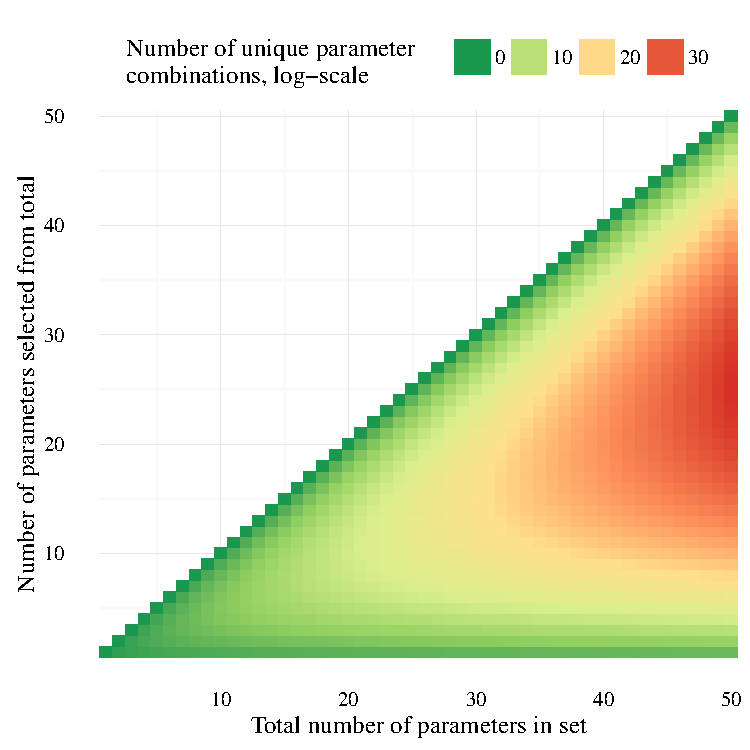
\includegraphics[width=0.6\textwidth]{figs/combnex-1} 

}

\caption[Examples of unique parameter combinations from different parameter sets and number of selected parameters]{Examples of unique parameter combinations from different parameter sets and number of selected parameters.  The number of combinations are shown for increasing numbers of selected parameters from the total in the set, where 50 parameter sets are shown each with one through 50 total parameters. Note that the number of unique combinations is shown as the natural-log.}\label{fig:combnex}
\end{figure}



\begin{figure}[!ht]

{\centering 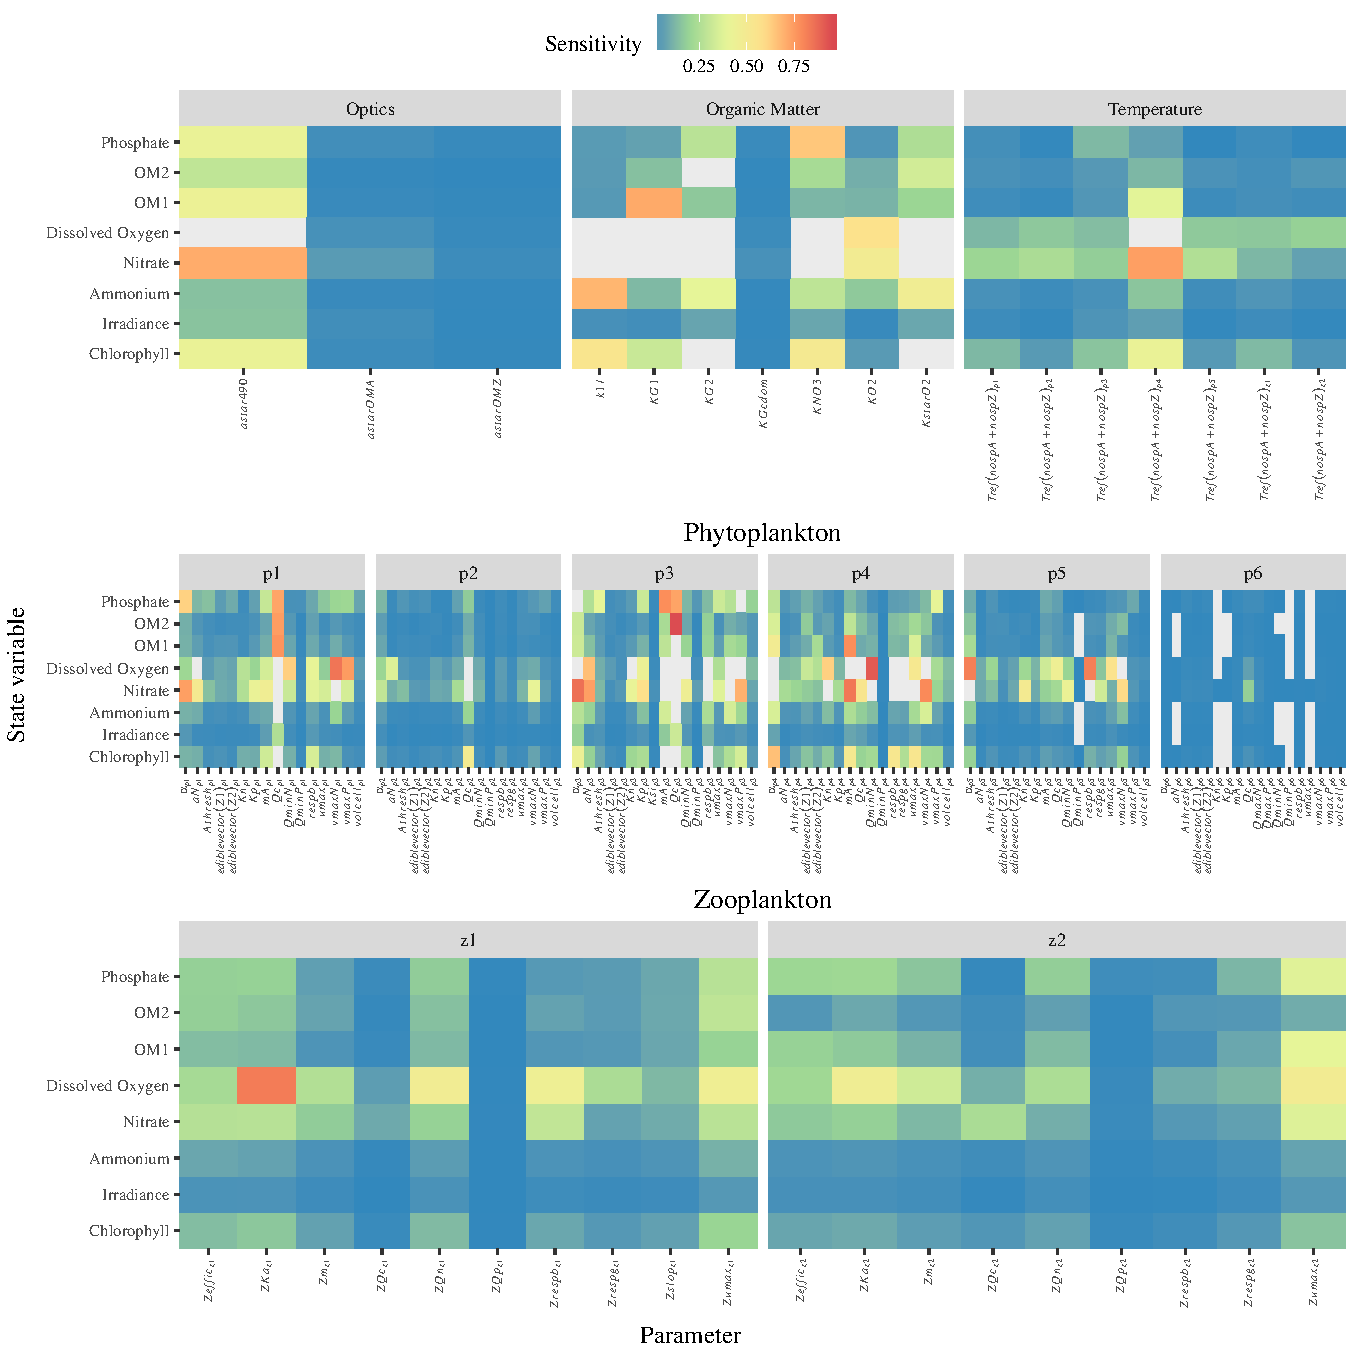
\includegraphics[width=\textwidth]{figs/sensalltile-1} 

}

\caption{Sensitivity values (L1, \cref{l1}) for local analyses of all state variables. Parameters are grouped by category: optics, organic matter, phytoplankton, zooplankton, temperature, and zoplankton.  See \cref{tab:dosens} for L1 values for \ac{do} and \cref{tab:nh4sens,tab:chlsens,tab:irrsens,tab:no3sens,tab:om1sens,tab:om2sens,tab:po4sens} for the other state variables.}\label{fig:sensalltile}
\end{figure}



% identifiability boxplots
\begin{figure}[!ht]

{\centering 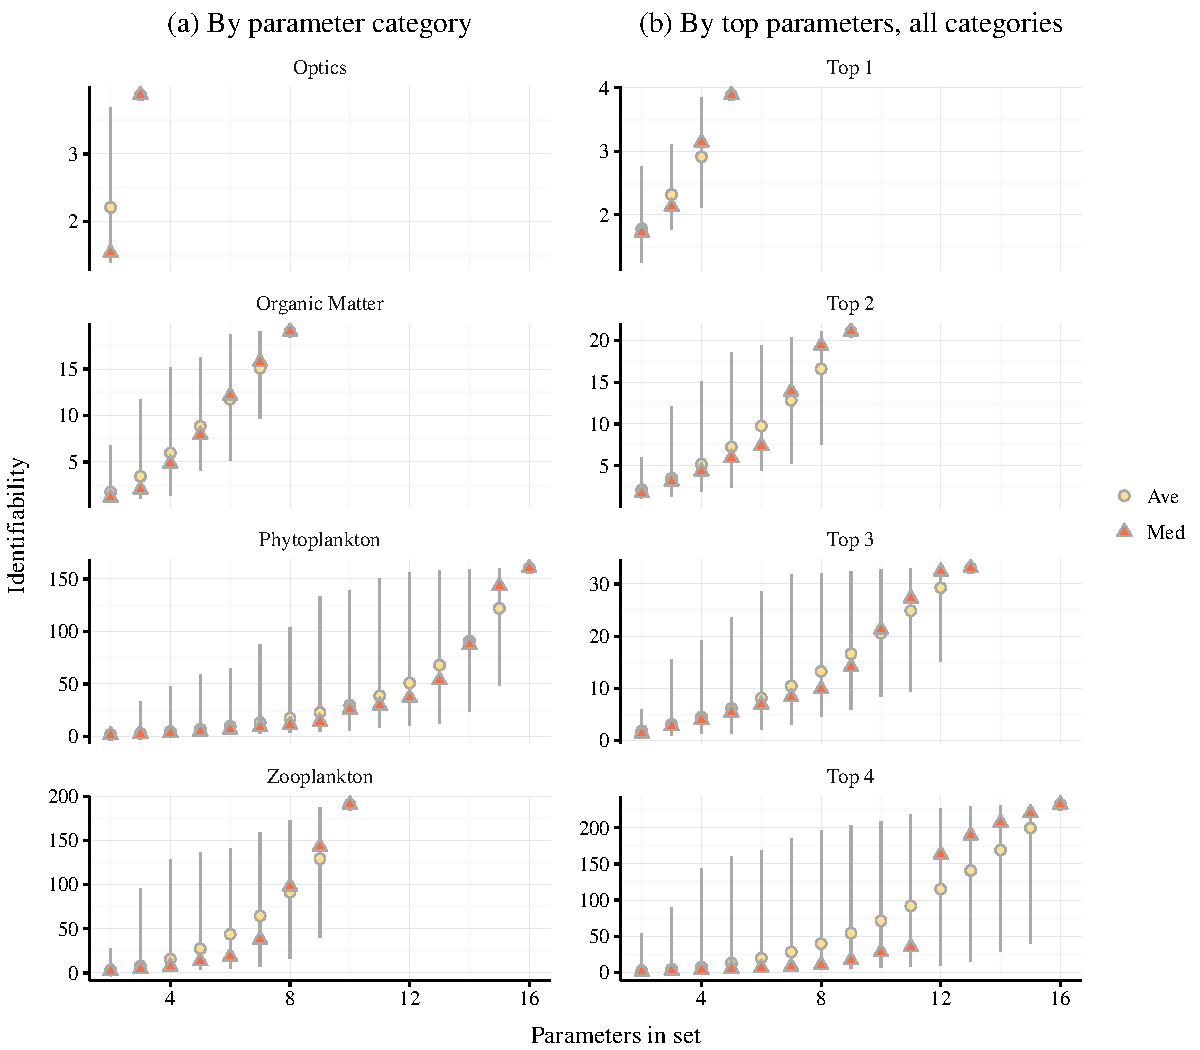
\includegraphics[width=\maxwidth]{figs/identbox-1} 

}

\caption{Identifiability (as $\gamma$, \cref{gameq}) of parameter subsets for \ac{do}.  Plots in (a) show identifiability by parameter categories and (b) shows identifiability by selecting the top 1 through 4 parameters in all categories.  Lines represent identifiability ranges for the possible combinations given the number of parameters in the set.  The temperature category is not shown because only \ac{do} was senstive to only one parameter.}\label{fig:identbox}
\end{figure}



% parameter exclusion temp
\begin{figure}[!ht]

{\centering 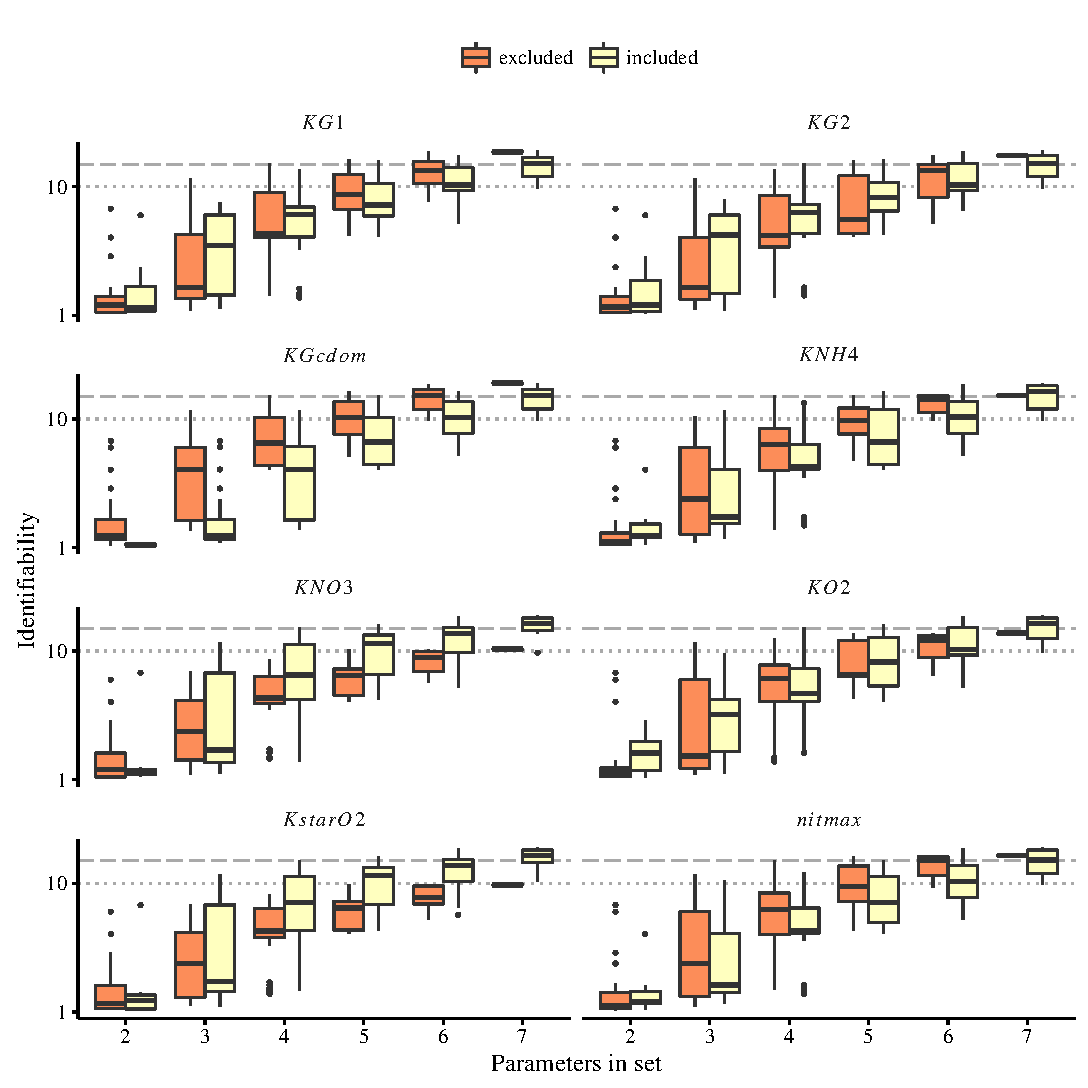
\includegraphics[width=\textwidth]{figs/exclex-1} 

}

\caption{Identifiability (as $\gamma$, \cref{gameq}) of organic matter parameters for subset combinations in \cref{fig:identbox}.  Identifiability is evaluated for subsets that excluded and included the parameters at the top of each plot. Identifiability of including all eight parameters is in \cref{fig:identbox}. Grey lines indicate potential thresholds at $\gamma = 10, 15$ for maximum acceptable identifiability.}\label{fig:exclex}
\end{figure}



% heuristic plots, all state
\begin{figure}[!ht]

{\centering 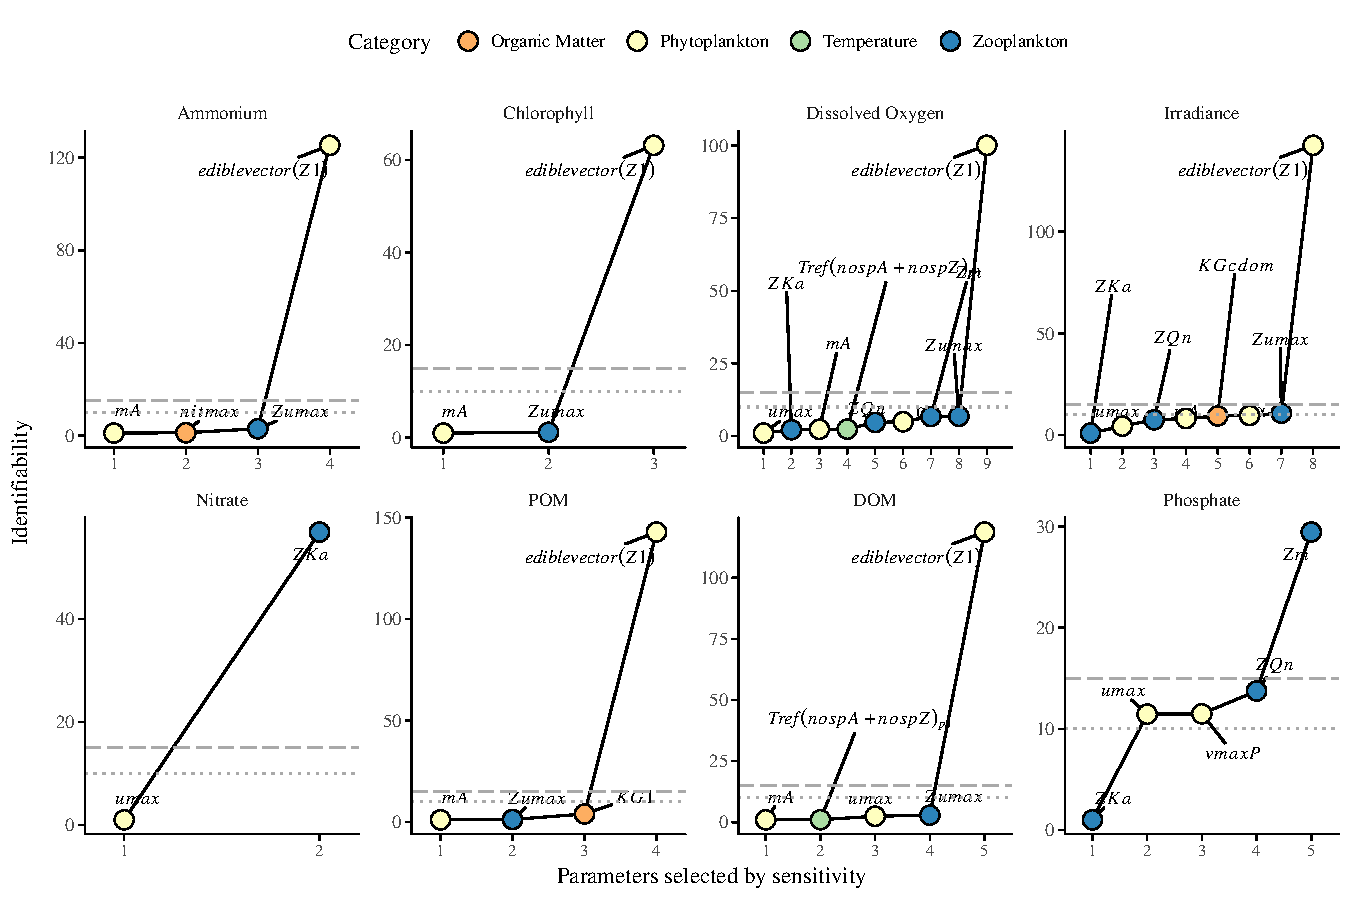
\includegraphics[width=\textwidth]{figs/heurist_stts-1} 

}

\caption[Identifiability (as ]{Identifiability (as $\gamma$, \cref{gameq}) of selecting parameters for all state variables. Parameters are selected by decreasing sensitivity independent of parameter categories. Grey lines indicate potential thresholds at $\gamma = 10, 15$ for maximum acceptable identifiability. Selection stops after $\gamma > 15$.}\label{fig:heurist_stts}
\end{figure}


\clearpage

% supplementary material
\beginsupplement

% ammonium sensitivity all categories
%latex.default(totab, file = "", rowlabel = "Description", caption = cap.val,     caption.loc = "top", rowname = Description, rgroup = unique(cats),     n.rgroup = as.numeric(table(cats)), size = tabsize, label = paste0("tab:",         tablab))%
\begin{table}[!tbp]
{\footnotesize
\caption{Sensitivity of ammonium to perturbations of indivividual parameters.  Sensitivities are based on a 50\% increase from the initial parameter value, where $L1$ summarizes differences in model output from the default (see \cref{l1}).  Parameters that did not affect ammonium are not shown.  Parameters are grouped by categories as optics, temperature, phytoplankton, zooplankton, and organic matter.\label{tab:nh4sens}} 
\begin{center}
\begin{tabular}{llll}
\hline\hline
\multicolumn{1}{l}{Description}&\multicolumn{1}{c}{Parameter}&\multicolumn{1}{c}{Value}&\multicolumn{1}{c}{L1}\tabularnewline
\hline
{\bfseries Optics}&&&\tabularnewline
~~OMA specific absorption at 490 nm&\textit{astarOMA}&$0.1$&$0.01$\tabularnewline
~~Chla specific absorption at 490 nm&\textit{astar490}&$0.04$&$0.01$\tabularnewline
~~OMZ specific absorption at 490 nm&\textit{astarOMZ}&$0.1$&$4.77\times 10^{-5}$\tabularnewline
\hline
{\bfseries Temperature}&&&\tabularnewline
~~Optimum temperature for growth(C)&\textit{Tref(nospA+nospZ)}&$22$&$0.61$\tabularnewline
\hline
{\bfseries Phytoplankton}&&&\tabularnewline
~~initial slope of the photosynthesis-irradiance relationship&\textit{alpha}&$8.42\times 10^{-17}$&$43.95$\tabularnewline
~~maximum growth rate&\textit{umax}&$0.41$&$9.63$\tabularnewline
~~mortality coefficient&\textit{mA}&$0.1$&$1.32$\tabularnewline
~~phytoplankton basal respiration coefficient&\textit{respb}&$0.02$&$0.9$\tabularnewline
~~N-uptake rate measured at umax&\textit{vmaxN}&$4.1\times 10^{-8}$&$0.56$\tabularnewline
~~coefficient for non-limiting nutrient&\textit{aN}&$1$&$0.31$\tabularnewline
~~half-saturation constant for P&\textit{Kp}&$2.86$&$0.3$\tabularnewline
~~phytoplankton growth respiration coefficient&\textit{respg}&$0.1$&$0.21$\tabularnewline
~~minimum N cell-quota&\textit{QminN}&$6.08\times 10^{-9}$&$0.05$\tabularnewline
~~half-saturation constant for N&\textit{Kn}&$4.51$&$0.04$\tabularnewline
~~phytoplankton carbon/cell&\textit{Qc}&$1.35\times 10^{-6}$&$0.02$\tabularnewline
~~P-uptake rate measured at umax&\textit{vmaxP}&$2.68\times 10^{-8}$&$9.3\times 10^{-3}$\tabularnewline
~~minimum P cell-quota&\textit{QminP}&$6.19\times 10^{-10}$&$6.4\times 10^{-3}$\tabularnewline
\hline
{\bfseries Zooplankton}&&&\tabularnewline
~~zooplankton nitrogen/individual&\textit{ZQn}&$6.95\times 10^{-5}$&$0.18$\tabularnewline
~~Zooplankton biomass-dependent respiration factor&\textit{Zrespb}&$0.1$&$0.17$\tabularnewline
~~Zooplankton mortality constant for quadratic mortality&\textit{Zm}&$7.2\times 10^{-4}$&$1.41\times 10^{-3}$\tabularnewline
~~zooplankton phosphorus/individual&\textit{ZQp}&$3.77\times 10^{-6}$&$1\times 10^{-3}$\tabularnewline
~~zooplankton carbon/individual&\textit{ZQc}&$3.13\times 10^{-4}$&$1.85\times 10^{-4}$\tabularnewline
\hline
{\bfseries Organic Matter}&&&\tabularnewline
~~NH4 rate constant for nitrification&\textit{KNH4}&$1$&$1.1$\tabularnewline
~~maximum rate of nitrification per day&\textit{nitmax}&$0.52$&$0.71$\tabularnewline
~~decay rate of CDOM, 1/day&\textit{KGcdom}&$0.01$&$0.36$\tabularnewline
~~turnover rate for OM1A and OM1G&\textit{KG1}&$50$&$0.2$\tabularnewline
~~half-saturation concentration for O2 utilization&\textit{KO2}&$10$&$0.14$\tabularnewline
~~O2 concentration that inhibits denitrification&\textit{KstarO2}&$10$&$0.07$\tabularnewline
~~turnover rate for OM2A and OM2G&\textit{KG2}&$50$&$0.05$\tabularnewline
~~half-saturation concentration for NO3 used in denitrification&\textit{KNO3}&$10$&$0.01$\tabularnewline
\hline
\end{tabular}\end{center}}

\end{table}


% chlorophyll sensitivity all categories
%latex.default(totab, file = "", rowlabel = "Description", caption = cap.val,     caption.loc = "top", rowname = Description, rgroup = unique(cats),     n.rgroup = as.numeric(table(cats)), size = tabsize, label = paste0("tab:",         tablab))%
\begin{table}[!tbp]
{\footnotesize
\caption{Sensitivity of \ac{chla} to perturbations of indivividual parameters.  Sensitivities are based on a 50\% increase from the initial parameter value, where $L1$ summarizes differences in model output from the default (see \cref{l1}).  Parameters that did not affect \ac{chla} are not shown.  Parameters are grouped by categories as optics, temperature, phytoplankton, zooplankton, and organic matter.\label{tab:chlsens}} 
\begin{center}
\begin{tabular}{llll}
\hline\hline
\multicolumn{1}{l}{Description}&\multicolumn{1}{c}{Parameter}&\multicolumn{1}{c}{Value}&\multicolumn{1}{c}{L1}\tabularnewline
\hline
{\bfseries Optics}&&&\tabularnewline
~~OMA specific absorption at 490 nm&\textit{astarOMA}&$0.1$&$0.02$\tabularnewline
~~Chla specific absorption at 490 nm&\textit{astar490}&$0.04$&$0.02$\tabularnewline
~~OMZ specific absorption at 490 nm&\textit{astarOMZ}&$0.1$&$6.77\times 10^{-5}$\tabularnewline
\hline
{\bfseries Temperature}&&&\tabularnewline
~~Optimum temperature for growth(C)&\textit{Tref(nospA+nospZ)}&$22$&$0.96$\tabularnewline
\hline
{\bfseries Phytoplankton}&&&\tabularnewline
~~initial slope of the photosynthesis-irradiance relationship&\textit{alpha}&$8.42\times 10^{-17}$&$132.89$\tabularnewline
~~maximum growth rate&\textit{umax}&$0.41$&$20.34$\tabularnewline
~~mortality coefficient&\textit{mA}&$0.1$&$1.9$\tabularnewline
~~phytoplankton basal respiration coefficient&\textit{respb}&$0.02$&$1.33$\tabularnewline
~~phytoplankton carbon/cell&\textit{Qc}&$1.35\times 10^{-6}$&$0.91$\tabularnewline
~~phytoplankton growth respiration coefficient&\textit{respg}&$0.1$&$0.37$\tabularnewline
~~minimum N cell-quota&\textit{QminN}&$6.08\times 10^{-9}$&$4.69\times 10^{-3}$\tabularnewline
~~half-saturation constant for P&\textit{Kp}&$2.86$&$2.25\times 10^{-3}$\tabularnewline
~~coefficient for non-limiting nutrient&\textit{aN}&$1$&$2.13\times 10^{-3}$\tabularnewline
~~N-uptake rate measured at umax&\textit{vmaxN}&$4.1\times 10^{-8}$&$7.11\times 10^{-4}$\tabularnewline
~~half-saturation constant for N&\textit{Kn}&$4.51$&$2.05\times 10^{-4}$\tabularnewline
~~P-uptake rate measured at umax&\textit{vmaxP}&$2.68\times 10^{-8}$&$1.71\times 10^{-4}$\tabularnewline
~~minimum P cell-quota&\textit{QminP}&$6.19\times 10^{-10}$&$2.32\times 10^{-5}$\tabularnewline
\hline
{\bfseries Zooplankton}&&&\tabularnewline
~~zooplankton carbon/individual&\textit{ZQc}&$3.13\times 10^{-4}$&$6.79\times 10^{-5}$\tabularnewline
~~Zooplankton biomass-dependent respiration factor&\textit{Zrespb}&$0.1$&$1.46\times 10^{-5}$\tabularnewline
~~Zooplankton mortality constant for quadratic mortality&\textit{Zm}&$7.2\times 10^{-4}$&$1.07\times 10^{-5}$\tabularnewline
~~zooplankton phosphorus/individual&\textit{ZQp}&$3.77\times 10^{-6}$&$6.48\times 10^{-6}$\tabularnewline
\hline
{\bfseries Organic Matter}&&&\tabularnewline
~~decay rate of CDOM, 1/day&\textit{KGcdom}&$0.01$&$0.58$\tabularnewline
~~turnover rate for OM1A and OM1G&\textit{KG1}&$50$&$0.02$\tabularnewline
~~half-saturation concentration for O2 utilization&\textit{KO2}&$10$&$1.69\times 10^{-3}$\tabularnewline
~~O2 concentration that inhibits denitrification&\textit{KstarO2}&$10$&$1.38\times 10^{-3}$\tabularnewline
~~half-saturation concentration for NO3 used in denitrification&\textit{KNO3}&$10$&$1.96\times 10^{-4}$\tabularnewline
~~turnover rate for OM2A and OM2G&\textit{KG2}&$50$&$3.14\times 10^{-5}$\tabularnewline
\hline
\end{tabular}\end{center}}

\end{table}


% irradiance sensitivity all categories
%latex.default(totab, file = "", rowlabel = "Description", caption = cap.val,     caption.loc = "top", rowname = Description, rgroup = unique(cats),     n.rgroup = as.numeric(table(cats)), size = tabsize, label = paste0("tab:",         tablab))%
\begin{table}[!tbp]
{\footnotesize
\caption{Sensitivity of irradiance to perturbations of indivividual parameters.  Sensitivities are based on a 50\% increase from the initial parameter value, where $L1$ summarizes differences in model output from the default (see \cref{l1}).  Parameters that did not affect irradiance are not shown.  Parameters are grouped by categories as optics, temperature, phytoplankton, zooplankton, and organic matter.\label{tab:irrsens}} 
\begin{center}
\begin{tabular}{llll}
\hline\hline
\multicolumn{1}{l}{Description}&\multicolumn{1}{c}{Parameter}&\multicolumn{1}{c}{Value}&\multicolumn{1}{c}{L1}\tabularnewline
\hline
{\bfseries Optics}&&&\tabularnewline
~~Chla specific absorption at 490 nm&\textit{astar490}&$0.04$&$2.71\times 10^{-3}$\tabularnewline
~~OMA specific absorption at 490 nm&\textit{astarOMA}&$0.1$&$2.41\times 10^{-3}$\tabularnewline
~~OMZ specific absorption at 490 nm&\textit{astarOMZ}&$0.1$&$7.15\times 10^{-6}$\tabularnewline
\hline
{\bfseries Temperature}&&&\tabularnewline
~~Optimum temperature for growth(C)&\textit{Tref(nospA+nospZ)}&$22$&$2.29\times 10^{-4}$\tabularnewline
\hline
{\bfseries Phytoplankton}&&&\tabularnewline
~~phytoplankton carbon/cell&\textit{Qc}&$1.35\times 10^{-6}$&$8.09\times 10^{-3}$\tabularnewline
~~initial slope of the photosynthesis-irradiance relationship&\textit{alpha}&$8.42\times 10^{-17}$&$7.65\times 10^{-3}$\tabularnewline
~~mortality coefficient&\textit{mA}&$0.1$&$7.42\times 10^{-3}$\tabularnewline
~~phytoplankton basal respiration coefficient&\textit{respb}&$0.02$&$2.13\times 10^{-3}$\tabularnewline
~~maximum growth rate&\textit{umax}&$0.41$&$2.09\times 10^{-3}$\tabularnewline
~~minimum N cell-quota&\textit{QminN}&$6.08\times 10^{-9}$&$7.39\times 10^{-4}$\tabularnewline
~~N-uptake rate measured at umax&\textit{vmaxN}&$4.1\times 10^{-8}$&$5.74\times 10^{-4}$\tabularnewline
~~coefficient for non-limiting nutrient&\textit{aN}&$1$&$4.7\times 10^{-4}$\tabularnewline
~~half-saturation constant for P&\textit{Kp}&$2.86$&$4.44\times 10^{-4}$\tabularnewline
~~phytoplankton growth respiration coefficient&\textit{respg}&$0.1$&$6.64\times 10^{-5}$\tabularnewline
~~half-saturation constant for N&\textit{Kn}&$4.51$&$4.7\times 10^{-5}$\tabularnewline
~~P-uptake rate measured at umax&\textit{vmaxP}&$2.68\times 10^{-8}$&$3.48\times 10^{-5}$\tabularnewline
~~minimum P cell-quota&\textit{QminP}&$6.19\times 10^{-10}$&$2.45\times 10^{-6}$\tabularnewline
\hline
{\bfseries Zooplankton}&&&\tabularnewline
~~zooplankton carbon/individual&\textit{ZQc}&$3.13\times 10^{-4}$&$7.23\times 10^{-6}$\tabularnewline
~~Zooplankton biomass-dependent respiration factor&\textit{Zrespb}&$0.1$&$1.05\times 10^{-6}$\tabularnewline
~~Zooplankton mortality constant for quadratic mortality&\textit{Zm}&$7.2\times 10^{-4}$&$9.27\times 10^{-7}$\tabularnewline
~~zooplankton phosphorus/individual&\textit{ZQp}&$3.77\times 10^{-6}$&$4.47\times 10^{-7}$\tabularnewline
~~zooplankton nitrogen/individual&\textit{ZQn}&$6.95\times 10^{-5}$&$2.43\times 10^{-8}$\tabularnewline
\hline
{\bfseries Organic Matter}&&&\tabularnewline
~~decay rate of CDOM, 1/day&\textit{KGcdom}&$0.01$&$0.05$\tabularnewline
~~turnover rate for OM1A and OM1G&\textit{KG1}&$50$&$1.6\times 10^{-3}$\tabularnewline
~~half-saturation concentration for O2 utilization&\textit{KO2}&$10$&$1.61\times 10^{-4}$\tabularnewline
~~O2 concentration that inhibits denitrification&\textit{KstarO2}&$10$&$1.31\times 10^{-4}$\tabularnewline
~~half-saturation concentration for NO3 used in denitrification&\textit{KNO3}&$10$&$1.82\times 10^{-5}$\tabularnewline
~~turnover rate for OM2A and OM2G&\textit{KG2}&$50$&$2.95\times 10^{-6}$\tabularnewline
~~NH4 rate constant for nitrification&\textit{KNH4}&$1$&$7.41\times 10^{-9}$\tabularnewline
~~maximum rate of nitrification per day&\textit{nitmax}&$0.52$&$4.81\times 10^{-9}$\tabularnewline
\hline
\end{tabular}\end{center}}

\end{table}


% nitrate sensitivity all categories
%latex.default(totab, file = "", rowlabel = "Description", caption = cap.val,     caption.loc = "top", rowname = Description, rgroup = unique(cats),     n.rgroup = as.numeric(table(cats)), size = tabsize, label = paste0("tab:",         tablab))%
\begin{table}[!tbp]
{\footnotesize
\caption{Sensitivity of nitrate to perturbations of indivividual parameters.  Sensitivities are based on a 50\% increase from the initial parameter value, where $L1$ summarizes differences in model output from the default (see \cref{l1}).  Parameters that did not affect nitrate are not shown.  Parameters are grouped by categories as optics, temperature, phytoplankton, zooplankton, and organic matter.\label{tab:no3sens}} 
\begin{center}
\begin{tabular}{llll}
\hline\hline
\multicolumn{1}{l}{Description}&\multicolumn{1}{c}{Parameter}&\multicolumn{1}{c}{Value}&\multicolumn{1}{c}{L1}\tabularnewline
\hline
{\bfseries Optics}&&&\tabularnewline
~~Chla specific absorption at 490 nm&\textit{astar490}&$0.04$&$5.03\times 10^{-4}$\tabularnewline
~~OMA specific absorption at 490 nm&\textit{astarOMA}&$0.1$&$2.58\times 10^{-4}$\tabularnewline
~~OMZ specific absorption at 490 nm&\textit{astarOMZ}&$0.1$&$8.38\times 10^{-7}$\tabularnewline
\hline
{\bfseries Temperature}&&&\tabularnewline
~~Optimum temperature for growth(C)&\textit{Tref(nospA+nospZ)}&$22$&$1.79\times 10^{-6}$\tabularnewline
\hline
{\bfseries Phytoplankton}&&&\tabularnewline
~~phytoplankton carbon/cell&\textit{Qc}&$1.35\times 10^{-6}$&$0.1$\tabularnewline
~~initial slope of the photosynthesis-irradiance relationship&\textit{alpha}&$8.42\times 10^{-17}$&$0.02$\tabularnewline
~~phytoplankton basal respiration coefficient&\textit{respb}&$0.02$&$9.21\times 10^{-3}$\tabularnewline
~~mortality coefficient&\textit{mA}&$0.1$&$8.6\times 10^{-3}$\tabularnewline
~~minimum N cell-quota&\textit{QminN}&$6.08\times 10^{-9}$&$4.69\times 10^{-3}$\tabularnewline
~~maximum growth rate&\textit{umax}&$0.41$&$4.56\times 10^{-3}$\tabularnewline
~~N-uptake rate measured at umax&\textit{vmaxN}&$4.1\times 10^{-8}$&$3.7\times 10^{-3}$\tabularnewline
~~coefficient for non-limiting nutrient&\textit{aN}&$1$&$1.91\times 10^{-3}$\tabularnewline
~~half-saturation constant for P&\textit{Kp}&$2.86$&$1.81\times 10^{-3}$\tabularnewline
~~half-saturation constant for N&\textit{Kn}&$4.51$&$1.54\times 10^{-4}$\tabularnewline
~~P-uptake rate measured at umax&\textit{vmaxP}&$2.68\times 10^{-8}$&$8.37\times 10^{-5}$\tabularnewline
~~minimum P cell-quota&\textit{QminP}&$6.19\times 10^{-10}$&$4.18\times 10^{-5}$\tabularnewline
\hline
{\bfseries Zooplankton}&&&\tabularnewline
~~zooplankton nitrogen/individual&\textit{ZQn}&$6.95\times 10^{-5}$&$1.28\times 10^{-3}$\tabularnewline
~~zooplankton carbon/individual&\textit{ZQc}&$3.13\times 10^{-4}$&$4.96\times 10^{-4}$\tabularnewline
~~Zooplankton mortality constant for quadratic mortality&\textit{Zm}&$7.2\times 10^{-4}$&$3.02\times 10^{-5}$\tabularnewline
~~Zooplankton biomass-dependent respiration factor&\textit{Zrespb}&$0.1$&$1.53\times 10^{-5}$\tabularnewline
~~zooplankton phosphorus/individual&\textit{ZQp}&$3.77\times 10^{-6}$&$5.55\times 10^{-6}$\tabularnewline
\hline
{\bfseries Organic Matter}&&&\tabularnewline
~~O2 concentration that inhibits denitrification&\textit{KstarO2}&$10$&$0.05$\tabularnewline
~~half-saturation concentration for NO3 used in denitrification&\textit{KNO3}&$10$&$7.09\times 10^{-3}$\tabularnewline
~~half-saturation concentration for O2 utilization&\textit{KO2}&$10$&$4.36\times 10^{-3}$\tabularnewline
~~turnover rate for OM1A and OM1G&\textit{KG1}&$50$&$1.5\times 10^{-3}$\tabularnewline
~~turnover rate for OM2A and OM2G&\textit{KG2}&$50$&$8.65\times 10^{-4}$\tabularnewline
~~decay rate of CDOM, 1/day&\textit{KGcdom}&$0.01$&$7.43\times 10^{-4}$\tabularnewline
~~maximum rate of nitrification per day&\textit{nitmax}&$0.52$&$3.34\times 10^{-4}$\tabularnewline
~~NH4 rate constant for nitrification&\textit{KNH4}&$1$&$3.23\times 10^{-4}$\tabularnewline
\hline
\end{tabular}\end{center}}

\end{table}


% om1 sensitivity all categories
%latex.default(totab, file = "", rowlabel = "Description", caption = cap.val,     caption.loc = "top", rowname = Description, rgroup = unique(cats),     n.rgroup = as.numeric(table(cats)), size = tabsize, label = paste0("tab:",         tablab))%
\begin{table}[!tbp]
{\footnotesize
\caption{Sensitivity of particulate organic matter to perturbations of indivividual parameters.  Sensitivities are based on a 50\% increase from the initial parameter value, where $L1$ summarizes differences in model output from the default (see \cref{l1}).  Parameters that did not affect particulate organic matter are not shown.  Parameters are grouped by categories as optics, temperature, phytoplankton, zooplankton, and organic matter.\label{tab:om1sens}} 
\begin{center}
\begin{tabular}{llll}
\hline\hline
\multicolumn{1}{l}{Description}&\multicolumn{1}{c}{Parameter}&\multicolumn{1}{c}{Value}&\multicolumn{1}{c}{L1}\tabularnewline
\hline
{\bfseries Optics}&&&\tabularnewline
~~OMA specific absorption at 490 nm&\textit{astarOMA}&$0.1$&$0.02$\tabularnewline
~~Chla specific absorption at 490 nm&\textit{astar490}&$0.04$&$0.02$\tabularnewline
~~OMZ specific absorption at 490 nm&\textit{astarOMZ}&$0.1$&$5.94\times 10^{-5}$\tabularnewline
\hline
{\bfseries Temperature}&&&\tabularnewline
~~Optimum temperature for growth(C)&\textit{Tref(nospA+nospZ)}&$22$&$0.92$\tabularnewline
\hline
{\bfseries Phytoplankton}&&&\tabularnewline
~~initial slope of the photosynthesis-irradiance relationship&\textit{alpha}&$8.42\times 10^{-17}$&$102.96$\tabularnewline
~~maximum growth rate&\textit{umax}&$0.41$&$18.21$\tabularnewline
~~mortality coefficient&\textit{mA}&$0.1$&$1.62$\tabularnewline
~~phytoplankton basal respiration coefficient&\textit{respb}&$0.02$&$1.2$\tabularnewline
~~phytoplankton carbon/cell&\textit{Qc}&$1.35\times 10^{-6}$&$0.95$\tabularnewline
~~phytoplankton growth respiration coefficient&\textit{respg}&$0.1$&$0.35$\tabularnewline
~~minimum N cell-quota&\textit{QminN}&$6.08\times 10^{-9}$&$0.16$\tabularnewline
~~N-uptake rate measured at umax&\textit{vmaxN}&$4.1\times 10^{-8}$&$0.1$\tabularnewline
~~coefficient for non-limiting nutrient&\textit{aN}&$1$&$0.09$\tabularnewline
~~half-saturation constant for P&\textit{Kp}&$2.86$&$0.09$\tabularnewline
~~half-saturation constant for N&\textit{Kn}&$4.51$&$8.86\times 10^{-3}$\tabularnewline
~~P-uptake rate measured at umax&\textit{vmaxP}&$2.68\times 10^{-8}$&$3.49\times 10^{-3}$\tabularnewline
~~minimum P cell-quota&\textit{QminP}&$6.19\times 10^{-10}$&$1.09\times 10^{-3}$\tabularnewline
\hline
{\bfseries Zooplankton}&&&\tabularnewline
~~zooplankton carbon/individual&\textit{ZQc}&$3.13\times 10^{-4}$&$1.87\times 10^{-3}$\tabularnewline
~~Zooplankton mortality constant for quadratic mortality&\textit{Zm}&$7.2\times 10^{-4}$&$1.1\times 10^{-3}$\tabularnewline
~~zooplankton phosphorus/individual&\textit{ZQp}&$3.77\times 10^{-6}$&$1.72\times 10^{-4}$\tabularnewline
~~Zooplankton biomass-dependent respiration factor&\textit{Zrespb}&$0.1$&$1.21\times 10^{-4}$\tabularnewline
~~zooplankton nitrogen/individual&\textit{ZQn}&$6.95\times 10^{-5}$&$2.19\times 10^{-5}$\tabularnewline
\hline
{\bfseries Organic Matter}&&&\tabularnewline
~~turnover rate for OM1A and OM1G&\textit{KG1}&$50$&$0.9$\tabularnewline
~~decay rate of CDOM, 1/day&\textit{KGcdom}&$0.01$&$0.53$\tabularnewline
~~half-saturation concentration for O2 utilization&\textit{KO2}&$10$&$0.15$\tabularnewline
~~O2 concentration that inhibits denitrification&\textit{KstarO2}&$10$&$0.11$\tabularnewline
~~half-saturation concentration for NO3 used in denitrification&\textit{KNO3}&$10$&$0.02$\tabularnewline
~~turnover rate for OM2A and OM2G&\textit{KG2}&$50$&$5.27\times 10^{-4}$\tabularnewline
~~maximum rate of nitrification per day&\textit{nitmax}&$0.52$&$3.67\times 10^{-6}$\tabularnewline
~~NH4 rate constant for nitrification&\textit{KNH4}&$1$&$1.75\times 10^{-6}$\tabularnewline
\hline
\end{tabular}\end{center}}

\end{table}


% om2 sensitivity all categories
%latex.default(totab, file = "", rowlabel = "Description", caption = cap.val,     caption.loc = "top", rowname = Description, rgroup = unique(cats),     n.rgroup = as.numeric(table(cats)), size = tabsize, label = paste0("tab:",         tablab))%
\begin{table}[!tbp]
{\footnotesize
\caption{Sensitivity of dissolved organic matter to perturbations of indivividual parameters.  Sensitivities are based on a 50\% increase from the initial parameter value, where $L1$ summarizes differences in model output from the default (see \cref{l1}).  Parameters that did not affect dissolved organic matter are not shown.  Parameters are grouped by categories as optics, temperature, phytoplankton, zooplankton, and organic matter.\label{tab:om2sens}} 
\begin{center}
\begin{tabular}{llll}
\hline\hline
\multicolumn{1}{l}{Description}&\multicolumn{1}{c}{Parameter}&\multicolumn{1}{c}{Value}&\multicolumn{1}{c}{L1}\tabularnewline
\hline
{\bfseries Optics}&&&\tabularnewline
~~OMA specific absorption at 490 nm&\textit{astarOMA}&$0.1$&$0.02$\tabularnewline
~~Chla specific absorption at 490 nm&\textit{astar490}&$0.04$&$0.02$\tabularnewline
~~OMZ specific absorption at 490 nm&\textit{astarOMZ}&$0.1$&$5.67\times 10^{-5}$\tabularnewline
\hline
{\bfseries Temperature}&&&\tabularnewline
~~Optimum temperature for growth(C)&\textit{Tref(nospA+nospZ)}&$22$&$0.96$\tabularnewline
\hline
{\bfseries Phytoplankton}&&&\tabularnewline
~~initial slope of the photosynthesis-irradiance relationship&\textit{alpha}&$8.42\times 10^{-17}$&$120$\tabularnewline
~~maximum growth rate&\textit{umax}&$0.41$&$19.66$\tabularnewline
~~mortality coefficient&\textit{mA}&$0.1$&$1.44$\tabularnewline
~~phytoplankton basal respiration coefficient&\textit{respb}&$0.02$&$1.09$\tabularnewline
~~phytoplankton carbon/cell&\textit{Qc}&$1.35\times 10^{-6}$&$0.96$\tabularnewline
~~minimum N cell-quota&\textit{QminN}&$6.08\times 10^{-9}$&$0.84$\tabularnewline
~~N-uptake rate measured at umax&\textit{vmaxN}&$4.1\times 10^{-8}$&$0.47$\tabularnewline
~~coefficient for non-limiting nutrient&\textit{aN}&$1$&$0.42$\tabularnewline
~~half-saturation constant for P&\textit{Kp}&$2.86$&$0.41$\tabularnewline
~~phytoplankton growth respiration coefficient&\textit{respg}&$0.1$&$0.34$\tabularnewline
~~half-saturation constant for N&\textit{Kn}&$4.51$&$0.04$\tabularnewline
~~P-uptake rate measured at umax&\textit{vmaxP}&$2.68\times 10^{-8}$&$9.43\times 10^{-3}$\tabularnewline
~~minimum P cell-quota&\textit{QminP}&$6.19\times 10^{-10}$&$6.95\times 10^{-3}$\tabularnewline
\hline
{\bfseries Zooplankton}&&&\tabularnewline
~~zooplankton carbon/individual&\textit{ZQc}&$3.13\times 10^{-4}$&$8.74\times 10^{-3}$\tabularnewline
~~Zooplankton mortality constant for quadratic mortality&\textit{Zm}&$7.2\times 10^{-4}$&$7.52\times 10^{-3}$\tabularnewline
~~zooplankton phosphorus/individual&\textit{ZQp}&$3.77\times 10^{-6}$&$1.1\times 10^{-3}$\tabularnewline
~~Zooplankton biomass-dependent respiration factor&\textit{Zrespb}&$0.1$&$2.72\times 10^{-4}$\tabularnewline
~~zooplankton nitrogen/individual&\textit{ZQn}&$6.95\times 10^{-5}$&$3.18\times 10^{-5}$\tabularnewline
\hline
{\bfseries Organic Matter}&&&\tabularnewline
~~turnover rate for OM2A and OM2G&\textit{KG2}&$50$&$0.98$\tabularnewline
~~decay rate of CDOM, 1/day&\textit{KGcdom}&$0.01$&$0.53$\tabularnewline
~~half-saturation concentration for O2 utilization&\textit{KO2}&$10$&$0.18$\tabularnewline
~~O2 concentration that inhibits denitrification&\textit{KstarO2}&$10$&$0.13$\tabularnewline
~~half-saturation concentration for NO3 used in denitrification&\textit{KNO3}&$10$&$0.02$\tabularnewline
~~turnover rate for OM1A and OM1G&\textit{KG1}&$50$&$0.01$\tabularnewline
~~maximum rate of nitrification per day&\textit{nitmax}&$0.52$&$1.14\times 10^{-5}$\tabularnewline
~~NH4 rate constant for nitrification&\textit{KNH4}&$1$&$6.11\times 10^{-6}$\tabularnewline
\hline
\end{tabular}\end{center}}

\end{table}


% phosphatesensitivity all categories
%latex.default(totab, file = "", rowlabel = "Description", caption = cap.val,     caption.loc = "top", rowname = Description, rgroup = unique(cats),     n.rgroup = as.numeric(table(cats)), size = tabsize, label = paste0("tab:",         tablab))%
\begin{table}[!tbp]
{\footnotesize
\caption{Sensitivity of phosphate to perturbations of indivividual parameters.  Sensitivities are based on a 50\% increase from the initial parameter value, where $L1$ summarizes differences in model output from the default (see \cref{l1}).  Parameters that did not affect phosphate are not shown.  Parameters are grouped by categories as optics, temperature, phytoplankton, zooplankton, and organic matter.\label{tab:po4sens}} 
\begin{center}
\begin{tabular}{llll}
\hline\hline
\multicolumn{1}{l}{Description}&\multicolumn{1}{c}{Parameter}&\multicolumn{1}{c}{Value}&\multicolumn{1}{c}{L1}\tabularnewline
\hline
{\bfseries Optics}&&&\tabularnewline
~~Chla specific absorption at 490 nm&\textit{astar490}&$0.04$&$2.08\times 10^{-4}$\tabularnewline
~~OMA specific absorption at 490 nm&\textit{astarOMA}&$0.1$&$8.92\times 10^{-5}$\tabularnewline
~~OMZ specific absorption at 490 nm&\textit{astarOMZ}&$0.1$&$2.09\times 10^{-6}$\tabularnewline
\hline
{\bfseries Temperature}&&&\tabularnewline
~~Optimum temperature for growth(C)&\textit{Tref(nospA+nospZ)}&$22$&$3.19\times 10^{-4}$\tabularnewline
\hline
{\bfseries Phytoplankton}&&&\tabularnewline
~~minimum P cell-quota&\textit{QminP}&$6.19\times 10^{-10}$&$0.02$\tabularnewline
~~mortality coefficient&\textit{mA}&$0.1$&$0.01$\tabularnewline
~~initial slope of the photosynthesis-irradiance relationship&\textit{alpha}&$8.42\times 10^{-17}$&$9.03\times 10^{-3}$\tabularnewline
~~P-uptake rate measured at umax&\textit{vmaxP}&$2.68\times 10^{-8}$&$7.23\times 10^{-3}$\tabularnewline
~~phytoplankton basal respiration coefficient&\textit{respb}&$0.02$&$5.4\times 10^{-3}$\tabularnewline
~~half-saturation constant for P&\textit{Kp}&$2.86$&$5.23\times 10^{-3}$\tabularnewline
~~maximum growth rate&\textit{umax}&$0.41$&$2.08\times 10^{-3}$\tabularnewline
~~phytoplankton carbon/cell&\textit{Qc}&$1.35\times 10^{-6}$&$3.87\times 10^{-4}$\tabularnewline
~~minimum N cell-quota&\textit{QminN}&$6.08\times 10^{-9}$&$1.63\times 10^{-4}$\tabularnewline
~~phytoplankton growth respiration coefficient&\textit{respg}&$0.1$&$1.13\times 10^{-4}$\tabularnewline
~~coefficient for non-limiting nutrient&\textit{aN}&$1$&$1.04\times 10^{-4}$\tabularnewline
~~N-uptake rate measured at umax&\textit{vmaxN}&$4.1\times 10^{-8}$&$8.56\times 10^{-5}$\tabularnewline
~~half-saturation constant for N&\textit{Kn}&$4.51$&$1.19\times 10^{-5}$\tabularnewline
\hline
{\bfseries Zooplankton}&&&\tabularnewline
~~zooplankton phosphorus/individual&\textit{ZQp}&$3.77\times 10^{-6}$&$2.99\times 10^{-3}$\tabularnewline
~~Zooplankton biomass-dependent respiration factor&\textit{Zrespb}&$0.1$&$6.74\times 10^{-5}$\tabularnewline
~~Zooplankton mortality constant for quadratic mortality&\textit{Zm}&$7.2\times 10^{-4}$&$6.68\times 10^{-6}$\tabularnewline
~~zooplankton carbon/individual&\textit{ZQc}&$3.13\times 10^{-4}$&$1.32\times 10^{-6}$\tabularnewline
~~zooplankton nitrogen/individual&\textit{ZQn}&$6.95\times 10^{-5}$&$3.59\times 10^{-7}$\tabularnewline
\hline
{\bfseries Organic Matter}&&&\tabularnewline
~~turnover rate for OM1A and OM1G&\textit{KG1}&$50$&$6.07\times 10^{-3}$\tabularnewline
~~turnover rate for OM2A and OM2G&\textit{KG2}&$50$&$2.38\times 10^{-3}$\tabularnewline
~~half-saturation concentration for O2 utilization&\textit{KO2}&$10$&$8.4\times 10^{-4}$\tabularnewline
~~O2 concentration that inhibits denitrification&\textit{KstarO2}&$10$&$7.05\times 10^{-4}$\tabularnewline
~~decay rate of CDOM, 1/day&\textit{KGcdom}&$0.01$&$3.73\times 10^{-4}$\tabularnewline
~~half-saturation concentration for NO3 used in denitrification&\textit{KNO3}&$10$&$1.01\times 10^{-4}$\tabularnewline
~~NH4 rate constant for nitrification&\textit{KNH4}&$1$&$2.44\times 10^{-7}$\tabularnewline
~~maximum rate of nitrification per day&\textit{nitmax}&$0.52$&$1.29\times 10^{-7}$\tabularnewline
\hline
\end{tabular}\end{center}}

\end{table}


\end{document}
